%%%%%%%%%%%%%%%%%%%%%%%%%%%%%%%%%%%%%%%%%%%%%%%%%%%%%%%%%%%%%%%%%%%%%%%%%%%%%%%%%%
   \begin{frame}[fragile]\frametitle{}
\begin{center}
{\Large Discrete Mathematics}

 - Sahil Mhaskar

\end{center}
\end{frame}

%%%%%%%%%%%%%%%%%%%%%%%%%%%%%%%%%%%%%%%%%%%%%%%%%%%%%%%%%%%
   \begin{frame}[fragile]{The Fibonacci sequence}

    \textit{The first two numbers in the Fibonacci sequence are 1 and 1. All
            other numbers in the sequence are defined as the sum of the previous two
            numbers in the sequence.}

    \begin{itemize}
        \item Task: Find the $n$th number in the Fibonacci sequence
        \item Let's solve this with dynamic programming
        \item Formulate the problem in terms of smaller versions of the problem (recursively)
    \end{itemize}

    \begin{align*}
        \mathrm{fibonacci}(1) &= 1\\
        \mathrm{fibonacci}(2) &= 1\\
        \mathrm{fibonacci}(n) &= \mathrm{fibonacci}(n - 2) + \mathrm{fibonacci}(n - 1)
    \end{align*}
\end{frame}

%%%%%%%%%%%%%%%%%%%%%%%%%%%%%%%%%%%%%%%%%%%%%%%%%%%%%%%%%%%
   \begin{frame}[fragile]{The Fibonacci sequence}
Turn this formulation into a recursive function


    \begin{lstlisting}
int fibonacci(int n) {
    if (n <= 2) {
        return 1;
    }

    int res = fibonacci(n - 2) + fibonacci(n - 1);

    return res;
}
    \end{lstlisting}
\end{frame}

% %%%%%%%%%%%%%%%%%%%%%%%%%%%%%%%%%%%%%%%%%%%%%%%%%%%%%%%%%%%
   % \begin{frame}[fragile]{The Fibonacci sequence}
% What is the time complexity of this?{Exponential, almost $O(2^n)$}


    % \begin{figure}

        % \begin{tikzpicture}

% [-,thick,%
  % every node/.style={shape=circle,draw,thick},%
  % level distance=0.5cm,
  % growth parent anchor={south}, nodes={anchor=north},
  % scale=0.8,%
% ]
% \scriptsize
% \node {$fib(6)$}
  % [sibling distance=5cm]
  % child {node {$fib(4)$}
    % [sibling distance=2cm]
    % child {node {$fib(2)$}
      % % [sibling distance=0.5cm]
      % % % child {node {$0$}}
      % % child {node {$fib(1)$}
      % %   % child {node {$0$}}
      % %   % child {node {$0$}}
      % % }
    % }
    % child {node {$fib(3)$}
      % [sibling distance=1cm]
      % child {node {$fib(1)$}
        % [sibling distance=0.5cm]
        % % child {node {$0$}}
        % % child {node {$0$}}
      % }
      % child {node {$fib(2)$}
        % % [sibling distance=0.5cm]
        % % % child {node {$0$}}
        % % child {node {$fib(1)$}
        % %   % child {node {$0$}}
        % %   % child {node {$0$}}
        % % }
      % }
    % }
  % }
  % child {node {$fib(5)$}
    % [sibling distance=3cm]
    % child {node {$fib(3)$}
      % [sibling distance=1cm]
      % child {node {$fib(1)$}
        % [sibling distance=0.5cm]
        % % child {node {$0$}}
        % % child {node {$0$}}
      % }
      % child {node {$fib(2)$}
        % % [sibling distance=0.5cm]
        % % % child {node {$0$}}
        % % child {node {$fib(1)$}
        % %   % child {node {$0$}}
        % %   % child {node {$0$}}
        % % }
      % }
    % }
    % child {node {$fib(4)$}
      % [sibling distance=2cm]
      % child {node {$fib(2)$}
        % % [sibling distance=0.5cm]
        % % % child {node {$0$}}
        % % child {node {$fib(1)$}
        % %   % child {node {$0$}}
        % %   % child {node {$0$}}
        % % }
      % }
      % child {node {$fib(3)$}
        % [sibling distance=1cm]
        % child {node {$fib(1)$}
          % [sibling distance=0.5cm]
          % % child {node {$0$}}
          % % child {node {$0$}}
        % }
        % child {node {$fib(2)$}
          % % [sibling distance=0.5cm]
          % % % child {node {$0$}}
          % % child {node {$fib(1)$}
          % %   % child {node {$0$}}
          % %   % child {node {$0$}}
          % % }
        % }
      % }
    % }
  % };
        % \end{tikzpicture}

% % \tikzset{
% %   treenode/.style = {align=center, inner sep=0pt, text centered,
% %     font=\sffamily},
% %   vertex/.style = {treenode, circle, white, font=\sffamily\bfseries\tiny, draw=white,
% %     text width=1.8em},% arbre rouge noir, noeud noir
% % }
% % 
% % \begin{tikzpicture}
% %     [->,>=stealth',level/.style={sibling distance = 5cm/#1,
% %   level distance = 1.8cm},scale=0.8] 
% %   \node [vertex] {fib(10)}
% %     child{ node [vertex] {fib(8)}
% %             child{ node [vertex] {fib(6)} 
% %                 child{ node [vertex] {fib(4)} }
% %                 child{ node [vertex] {fib(5)}}
% %             }
% %             child{ node [vertex] {fib(7)}
% %                             child{ node [vertex] {fib(5)}}
% %                             child{ node [vertex] {fib(6)}}
% %             }
% %     }
% %     child{ node [vertex] {fib(9)}
% %         child{ node [vertex] {fib(7)} 
% %             child{
% %                 node [vertex] {fib(5)}
% %                     child { node [vertex] {fib(3)} }
% %                     child { node [vertex] {fib(4)} }
% %                 }
% %             child{ node [vertex] {fib(6)}
% %             }
% %             }
% %             child{ node [vertex] {fib(8)}
% % 							child{ node [vertex] {49}}
% % 							% child{ node [vertex] {}}
% %             }
% % 		}
% % ; 
% % \end{tikzpicture}
            % \end{figure}

% \end{frame}

%%%%%%%%%%%%%%%%%%%%%%%%%%%%%%%%%%%%%%%%%%%%%%%%%%%%%%%%%%%
   \begin{frame}[fragile]{The Fibonacci sequence}
 Memoize the function (remember results that have been computed)
    \begin{lstlisting}
map<int, int> mem;

int fibonacci(int n) {
    if (n <= 2) {
        return 1;
    }

    if (mem.find(n) != mem.end()) {
        return mem[n];
    }

    int res = fibonacci(n - 2) + fibonacci(n - 1);

    mem[n] = res;
    return res;
}
    \end{lstlisting}

\end{frame}

%%%%%%%%%%%%%%%%%%%%%%%%%%%%%%%%%%%%%%%%%%%%%%%%%%%%%%%%%%%
   \begin{frame}[fragile]{The Fibonacci sequence}

    \begin{lstlisting}
int mem[1000];
for (int i = 0; i < 1000; i++)
    mem[i] = -1;

int fibonacci(int n) {
    if (n <= 2) {
        return 1;
    }

    if (mem[n] != -1) {
        return mem[n];
    }

    int res = fibonacci(n - 2) + fibonacci(n - 1);

    mem[n] = res;
    return res;
}
    \end{lstlisting}

\end{frame}

%%%%%%%%%%%%%%%%%%%%%%%%%%%%%%%%%%%%%%%%%%%%%%%%%%%%%%%%%%%
   \begin{frame}[fragile]{The Fibonacci sequence}
    \begin{itemize}
        \item What is the time complexity now?
        \item We have $n$ possible inputs to the function: $1$, $2$, \ldots, $n$.
        \item Each input will either:
            \begin{itemize}
                \item be computed, and the result saved
                \item be returned from memory
            \end{itemize}
        \item Each input will be computed at most once
        \item Time complexity is $O(n \times f)$, where $f$ is the time complexity of computing an input if we assume that the recursive calls are returned directly from memory ($O(1)$)
        \item Since we're only doing constant amount of work to compute the answer to an input, $f = O(1)$
        \item Total time complexity is $O(n)$
    \end{itemize}
\end{frame}

%%%%%%%%%%%%%%%%%%%%%%%%%%%%%%%%%%%%%%%%%%%%%%%%%%%%%%%%%%%
   \begin{frame}[fragile]\frametitle{Recap}
\begin{itemize}
\item Fibonacci: 1,1, 2, 3, 5, 8, 13, \ldots
\item $f_1 = 1, f_2 = 1, f_n = f_{n-1} + f_{n-2}$
\item Recursive:
\begin{lstlisting}
fib(n}{
	if n=1,2
		return 1
	else
		return fib(n-1) + fib(n-2)
}
\end{lstlisting}
\item Many computations are repeated.
\item Simple loop solution does not have this problem. Thats $O(n)$

\end{itemize}
\end{frame}

%%%%%%%%%%%%%%%%%%%%%%%%%%%%%%%%%%%%%%%%%%%%%%%%%%%%%%%%%%%
   \begin{frame}[fragile]{A Simple Loop for Fibonacci Numbers}


\begin{lstlisting}
function fib(n) {
  if (n <= 1) {
    return 1;
  } else {
    var last = 1, nextToLast = 1; answer = 1; 
    var i = 2;
    while (i <= n) {
      answer = last + nextToLast;
      nextToLast = last;
      last = answer;
      i = i + 1;
    }
    return answer;
} }
\end{lstlisting}
\end{frame}

%%%%%%%%%%%%%%%%%%%%%%%%%%%%%%%%%%%%%%%%%%%%%%%%%%%%%%%%%%%
   \begin{frame}[fragile]{Algorithm Design Techniques}

  \begin{enumerate}
  \item Goal: design efficient (polynomial-time) algorithms.
  \item Greedy
    \begin{itemize}
    \item Pro: natural approach to algorithm design.
    \item Con: many greedy approaches to a problem. Only some may work.
    \item Con: many problems for which \emph{no} greedy approach is known.
    \end{itemize}
  \end{enumerate}
\end{frame}

%%%%%%%%%%%%%%%%%%%%%%%%%%%%%%%%%%%%%%%%%%%%%%%%%%%%%%%%%%%
   \begin{frame}[fragile]{Algorithm Design Techniques}

  \begin{enumerate}
  \item Goal: design efficient (polynomial-time) algorithms.
  \item Divide and conquer
    \begin{itemize}
    \item Pro: simple to develop algorithm skeleton.
    \item Con: conquer step can be very hard to implement efficiently.
    \item Con: usually reduces time for a problem known to be solvable
      in polynomial time.    
    \end{itemize}
  \end{enumerate}
\end{frame}

%%%%%%%%%%%%%%%%%%%%%%%%%%%%%%%%%%%%%%%%%%%%%%%%%%%%%%%%%%%
   \begin{frame}[fragile]{Algorithm Design Techniques}

  \begin{enumerate}
  \item Goal: design efficient (polynomial-time) algorithms.
  \item Dynamic programming
    \begin{itemize}
    \item More powerful than greedy and divide-and-conquer strategies.
    \item \emph{Implicitly} explore space of all possible solutions.
    \item Solve multiple sub-problems and build up correct solutions to
      larger and larger sub-problems.
    \item Careful analysis needed to ensure number of sub-problems
      solved is polynomial in the size of the input.
    \end{itemize}
  \end{enumerate}
\end{frame}


%%%%%%%%%%%%%%%%%%%%%%%%%%%%%%%%%%%%%%%%%%%%%%%%%%%%%%%%%%%
   \begin{frame}[fragile]{What is dynamic programming?}
    \begin{itemize}
        \item A problem solving paradigm
        \item Similar in some respects to both divide and conquer and backtracking
        \item Divide and conquer recap:
            \begin{itemize}
                \item Split the problem into \textit{independent} subproblems
                \item Solve each subproblem recursively
                \item Combine the solutions to subproblems into a solution for the given problem
            \end{itemize}
        \item Dynamic programming:
            \begin{itemize}
                \item Split the problem into \textit{overlapping} subproblems
                \item Solve each subproblem recursively
                \item Combine the solutions to subproblems into a solution for the given problem
                \item \textit{Don't compute the answer to the same subproblem more than once}
            \end{itemize}
    \end{itemize}
\end{frame}

%%%%%%%%%%%%%%%%%%%%%%%%%%%%%%%%%%%%%%%%%%%%%%%%%%%%%%%%%%%
   \begin{frame}[fragile]{Dynamic programming formulation}

    \begin{itemize}
        \item Formulate the problem in terms of smaller versions of the problem (recursively)
        \item Turn this formulation into a recursive function
        \item Memorize the function (remember results that have been computed)
    \end{itemize}
\end{frame}

%%%%%%%%%%%%%%%%%%%%%%%%%%%%%%%%%%%%%%%%%%%%%%%%%%%%%%%%%%%
   \begin{frame}[fragile]{Basic Outline of Dynamic Programming}
  \begin{itemize}
  \item To solve a problem, we need a collection of sub-problems that
    satisfy a few properties:
    \begin{enumerate}
    \item There are a polynomial number of sub-problems.
    \item The solution to the problem can be computed easily from the
      solutions to the sub-problems.
    \item There is a natural ordering of the sub-problems from
      ``smallest'' to ``largest''.
    \item There is an easy-to-compute recurrence that allows us to
      compute the solution to a sub-problem from the solutions to some
      smaller sub-problems.
    \end{enumerate} 
  \item Difficulties in designing dynamic programming algorithms:
    \begin{enumerate}
    \item Which sub-problems to define?
    \item How can we tie together sub-problems using a recurrence?
    \item How do we order the sub-problems (to allow iterative
      computation of optimal solutions to sub-problems)?
    \end{enumerate}
  \end{itemize}
\end{frame}

%%%%%%%%%%%%%%%%%%%%%%%%%%%%%%%%%%%%%%%%%%%%%%%%%%%%%%%%%%%
   \begin{frame}[fragile]{Dynamic programming formulation}
    \begin{lstlisting}
map<problem, value> memory;

value dp(problem P) {
    if (is_base_case(P)) {
        return base_case_value(P);
    }

    if (memory.find(P) != memory.end()) {
        return memory[P];
    }

    value result = some value;
    for (problem Q in subproblems(P)) {
        result = combine(result, dp(Q));
    }

    memory[P] = result;
    return result;
}
    \end{lstlisting}
\end{frame}


%%%%%%%%%%%%%%%%%%%%%%%%%%%%%%%%%%%%%%%%%%%%%%%%%%%%%%%%%%%
   \begin{frame}[fragile]{History of Dynamic Programming}

  \begin{itemize}
  \item Bellman pioneered the systematic study of dynamic programming in
    the 1950s.  

%   \item Dynamic programming = ``planning over time.''
  \item The Secretary of Defense at that time was hostile to mathematical research.
  \item Bellman sought an impressive name to avoid confrontation. 
    \begin{itemize}
    \item ``it's impossible to use dynamic in a pejorative sense''
    \item ``something not even a Congressman could object to''
      (Ref:{(Bellman, R. E., \emph{Eye of the Hurricane, An
        Autobiography})}).
    \end{itemize} 
  \end{itemize}
\end{frame}

%%%%%%%%%%%%%%%%%%%%%%%%%%%%%%%%%%%%%%%%%%%%%%%%%%%%%%%%%%%
   \begin{frame}[fragile]{Applications of Dynamic Programming}

  \begin{itemize}
  \item Computational biology: Smith-Waterman algorithm for sequence alignment.
  \item Operations research: Bellman-Ford algorithm for shortest path
    routing in networks.
  \item Control theory: Viterbi algorithm for hidden Markov models.
  \item Computer science (theory, graphics, AI, \ldots): Unix
    \texttt{diff} command for comparing two files.
  \end{itemize}
\end{frame}


%%%%%%%%%%%%%%%%%%%%%%%%%%%%%%%%%%%%%%%%%%%%%%%%%%%%%%%%%%%
   \begin{frame}[fragile]{Maximum sum}
Given an array $\mathrm{arr}[0]$, $\mathrm{arr}[1]$, \ldots, $\mathrm{arr}[n-1]$ of integers, find the interval with the highest sum


    \begin{center}
        \begin{tabular}{|c|c|c|c|c|c|c|}
            \hline
            -15 & {8} & {-2} & {1} & {0} & {6} & -3 \\
            \hline
        \end{tabular}
    \end{center}

    \begin{itemize}
        \item The maximum sum of an interval in this array is $13$

        \item But how do we solve this in general?
            \begin{itemize}
        \item Easy to loop through all $\approx n^2$ intervals, and calculate their sums, but that is $O(n^3)$
        \item We could use our static range sum trick to get this down to $O(n^2)$
        \item Can we do better with dynamic programming?
            \end{itemize}
    \end{itemize}

\end{frame}

%%%%%%%%%%%%%%%%%%%%%%%%%%%%%%%%%%%%%%%%%%%%%%%%%%%%%%%%%%%
   \begin{frame}[fragile]{Maximum sum}

    \begin{itemize}
        \item First step is to formulate this recursively
        \item Let $\mathrm{max\_{}sum}(i)$ be the maximum sum interval in the range $0,\ldots,i$
        \item Base case: $\mathrm{max\_{}sum}(0) = \mathrm{max}(0, arr[0])$
        \item What about $\mathrm{max\_{}sum}(i)$?
        \item What does $\mathrm{max\_{}sum}(i-1)$ return?
        \item Is it possible to combine solutions to subproblems with smaller $i$ into a solution for $i$?
        \item At least it's not obvious...
    \end{itemize}

\end{frame}

%%%%%%%%%%%%%%%%%%%%%%%%%%%%%%%%%%%%%%%%%%%%%%%%%%%%%%%%%%%
   \begin{frame}[fragile]{Maximum sum}

    \begin{itemize}
        \item Let's try changing perspective

    \item Let $\mathrm{max\_{}sum}(i)$ be the maximum sum interval in the range $0,\ldots,i$, \textit{that ends at $i$}

        \item Base case: $\mathrm{max\_{}sum}(0) = arr[0]$

    \item $\mathrm{max\_{}sum}(i) = \mathrm{max}(arr[i], arr[i] + \mathrm{max\_{}sum}(i - 1))$

        \item Then the answer is just $\mathrm{max}_{\ 0 \leq i < n}\ \{\ \mathrm{max\_{}sum}(i)\ \}$
    \end{itemize}

\end{frame}

%%%%%%%%%%%%%%%%%%%%%%%%%%%%%%%%%%%%%%%%%%%%%%%%%%%%%%%%%%%
   \begin{frame}[fragile]{Maximum sum}
 Next step is to turn this into a function

    \begin{lstlisting}
int arr[1000];

int max_sum(int i) {
    if (i == 0) {
        return arr[i];
    }

    int res = max(arr[i], arr[i] + max_sum(i - 1));

    return res;
}
    \end{lstlisting}
\end{frame}

%%%%%%%%%%%%%%%%%%%%%%%%%%%%%%%%%%%%%%%%%%%%%%%%%%%%%%%%%%%
   \begin{frame}[fragile]{Maximum sum}
Final step is to memoize the function

    \begin{lstlisting}
int arr[1000];
int mem[1000];
bool comp[1000];
memset(comp, 0, sizeof(comp));

int max_sum(int i) {
    if (i == 0) {
        return arr[i];
    }
    if (comp[i]) {
        return mem[i];
    }

    int res = max(arr[i], arr[i] + max_sum(i - 1));

    mem[i] = res;
    comp[i] = true;
    return res;
}
    \end{lstlisting}
\end{frame}

%%%%%%%%%%%%%%%%%%%%%%%%%%%%%%%%%%%%%%%%%%%%%%%%%%%%%%%%%%%
   \begin{frame}[fragile]{Maximum sum}
Then the answer is just the maximum over all interval ends


    \begin{lstlisting}
int maximum = 0;
for (int i = 0; i < n; i++) {
    maximum = max(maximum, best_sum(i));
}

printf("%d\n", maximum);
    \end{lstlisting}
    If you want to find the maximum sum interval in multiple arrays, remember to clear the memory in between
\end{frame}

%%%%%%%%%%%%%%%%%%%%%%%%%%%%%%%%%%%%%%%%%%%%%%%%%%%%%%%%%%%
   \begin{frame}[fragile]{Maximum sum}
    \begin{itemize}
        \item What about time complexity?
        \item There are $n$ possible inputs to the function
        \item Each input is processed in $O(1)$ time, assuming recursive calls are $O(1)$
        \item Time complexity is $O(n)$
    \end{itemize}
\end{frame}

%%%%%%%%%%%%%%%%%%%%%%%%%%%%%%%%%%%%%%%%%%%%%%%%%%%%%%%%%%%
   \begin{frame}[fragile]{Coin change}
    \begin{itemize}
\item We have some amount, say, 37/-, split into coins, with aim to have minimum number of coins. 
\item Coins denomination available are 10, 5, 2, 1.
\item Greedy approach: Max first: 10,10,10,5,2. 
\item Greedy strategy: Subtract with max till possible, then the next max and so on.
\item For 23/- with coins as 1,4,5?
\item Greedy: 5 + 5 + 5 + 5 + 5 + 1 + 1 + 1. So, 7 coins.
\item But better solution would have been: 5 + 5+ 5+4+4. So, 5 coins.
    \end{itemize}
\end{frame}



%%%%%%%%%%%%%%%%%%%%%%%%%%%%%%%%%%%%%%%%%%%%%%%%%%%%%%%%%%%
   \begin{frame}[fragile]{Coin change}
    \begin{itemize}
\item Given an array of coin denominations $d_0$, $d_1$, \ldots, $d_{n-1}$,
            and some amount $x$: What is minimum number of coins needed to
            represent the value $x$?

        \item Remember the greedy algorithm for Coin change?
        \item It didn't always give the optimal solution, and sometimes it didn't even give a solution at all...

        \item What about dynamic programming?
    \end{itemize}
\end{frame}

%%%%%%%%%%%%%%%%%%%%%%%%%%%%%%%%%%%%%%%%%%%%%%%%%%%%%%%%%%%
   \begin{frame}[fragile]{Coin change}
    \begin{itemize}
        \item First step: formulate the problem recursively
\item Let $\mathrm{opt}(i,x)$ denote the minimum number of coins needed to represent the value $x$ if we're only allowed to use coin denominations $d_0$, \ldots, $d_i$
        \item Base case: $\mathrm{opt}(i,x) = \infty$ if $x < 0$
        \item Base case: $\mathrm{opt}(i,0) = 0$
        \item Base case: $\mathrm{opt}(-1,x) = \infty$
\item $\mathrm{opt}(i,x) = \mathrm{min} \left\{
	\begin{array}{l}
        1 + \mathrm{opt}(i, x - d_i) \\
        \mathrm{opt}(i-1, x)
	\end{array}
\right.$
    \end{itemize}
\end{frame}

%%%%%%%%%%%%%%%%%%%%%%%%%%%%%%%%%%%%%%%%%%%%%%%%%%%%%%%%%%%
   \begin{frame}[fragile]{Coin change}
    \begin{lstlisting}
int INF = 100000;
int d[10];

int opt(int i, int x) {
    if (x < 0) return INF;
    if (x == 0) return 0;
    if (i == -1) return INF;

    int res = INF;
    res = min(res, 1 + opt(i, x - d[i]));
    res = min(res, opt(i - 1, x));

    return res;
}
    \end{lstlisting}
\end{frame}

%%%%%%%%%%%%%%%%%%%%%%%%%%%%%%%%%%%%%%%%%%%%%%%%%%%%%%%%%%%
   \begin{frame}[fragile]{Coin change}
    \begin{lstlisting}
int INF = 100000;
int d[10];
int mem[10][10000];
memset(mem, -1, sizeof(mem));

int opt(int i, int x) {
    if (x < 0) return INF;
    if (x == 0) return 0;
    if (i == -1) return INF;

    if (mem[i][x] != -1) return mem[i][x];

    int res = INF;
    res = min(res, 1 + opt(i, x - d[i]));
    res = min(res, opt(i - 1, x));

    mem[i][x] = res;
    return res;
}
    \end{lstlisting}
\end{frame}

%%%%%%%%%%%%%%%%%%%%%%%%%%%%%%%%%%%%%%%%%%%%%%%%%%%%%%%%%%%
   \begin{frame}[fragile]{Coin change}
    \begin{itemize}
        \item Time complexity?
        \item Number of possible inputs are $n \times x$
        \item Each input will be processed in $O(1)$ time, assuming recursive calls are constant
        \item Total time complexity is $O(n\times x)$
    \end{itemize}
\end{frame}

%%%%%%%%%%%%%%%%%%%%%%%%%%%%%%%%%%%%%%%%%%%%%%%%%%%%%%%%%%%
   \begin{frame}[fragile]{Coin change}
    \begin{itemize}
        \item How do we know which coins the optimal solution used?
        \item We can store backpointers, or some extra information, to trace backwards through the states
        \item See example...
    \end{itemize}
\end{frame}

%%%%%%%%%%%%%%%%%%%%%%%%%%%%%%%%%%%%%%%%%%%%%%%%%%%%%%%%%%%
   \begin{frame}[fragile]{Longest increasing subsequence}
    \begin{itemize}
\item Given an array $a[0]$, $a[1]$, \ldots, $a[n-1]$ of integers, what is the length of the longest increasing subsequence?
\item First, what is a subsequence?
\item If we delete zero or more elements from $a$, then we have a subsequence of $a$
\item Example: $a = [5,1,8,1,9,2]$
\item $[5,8,9]$ is a subsequence
\item $[1,1]$ is a subsequence
\item $[5,1,8,1,9,2]$ is a subsequence
\item $[]$ is a subsequence
\item $[8,5]$ is \textbf{not} a subsequence
\item $[10]$ is \textbf{not} a subsequence
    \end{itemize}
\end{frame}

%%%%%%%%%%%%%%%%%%%%%%%%%%%%%%%%%%%%%%%%%%%%%%%%%%%%%%%%%%%
   \begin{frame}[fragile]{Longest increasing subsequence}
    \begin{itemize}
\item Given an array $a[0]$, $a[1]$, \ldots, $a[n-1]$ of integers, what is the length of the longest increasing subsequence?
\item An increasing subsequence of $a$ is a subsequence of $a$ such that the elements are in (strictly) increasing order

\item $[5,8,9]$ and $[1,8,9]$ are the longest increasing subsequences of $a = [5,1,8,1,9,2]$
\item How do we compute the length of the longest increasing subsequence?
\item There are $2^n$ subsequences, so we can go through all of them
\item That would result in an $O(n2^n)$ algorithm, which can only handle $n\leq 23$
\item What about dynamic programming?

    \end{itemize}
\end{frame}

%%%%%%%%%%%%%%%%%%%%%%%%%%%%%%%%%%%%%%%%%%%%%%%%%%%%%%%%%%%
   \begin{frame}[fragile]{Longest increasing subsequence}

    \begin{itemize}
\item Let $\mathrm{lis}(i)$ denote the length of the longest increasing subsequence of the array $a[0]$, $\ldots$, $a[i]$

\item Base case: $\mathrm{lis}(0) = 1$
\item What about $\mathrm{lis}(i)$?
\item We have the same issue as in the maximum sum problem, so let's try changing perspective
    \end{itemize}
\end{frame}

%%%%%%%%%%%%%%%%%%%%%%%%%%%%%%%%%%%%%%%%%%%%%%%%%%%%%%%%%%%
   \begin{frame}[fragile]{Longest increasing subsequence}

    \begin{itemize}
\item Let $\mathrm{lis}(i)$ denote the length of the longest increasing subsequence of the array $a[0]$, $\ldots$, $a[i]$, \textit{that ends at $i$}

\item Base case: we don't need one
\item $\mathrm{lis}(i) = \mathrm{max}(1, \mathrm{max}_{j<i \textrm{ s.t. } a[j] < a[i]} \{ 1 + \mathrm{lis}(j) \})$
    \end{itemize}
\end{frame}

%%%%%%%%%%%%%%%%%%%%%%%%%%%%%%%%%%%%%%%%%%%%%%%%%%%%%%%%%%%
   \begin{frame}[fragile]{Longest increasing subsequence}
    \begin{lstlisting}
int a[1000];
int mem[1000];
memset(mem, -1, sizeof(mem));

int lis(int i) {
    if (mem[i] != -1) {
        return mem[i];
    }

    int res = 1;
    for (int j = 0; j < i; j++) {
        if (a[j] < a[i]) {
            res = max(res, 1 + lis(j));
        }
    }

    mem[i] = res;
    return res;
}
    \end{lstlisting}
\end{frame}

%%%%%%%%%%%%%%%%%%%%%%%%%%%%%%%%%%%%%%%%%%%%%%%%%%%%%%%%%%%
   \begin{frame}[fragile]{Longest increasing subsequence}

    \begin{itemize}
        \item And then the longest increasing subsequence can be found by checking all endpoints:
    \end{itemize}

    \begin{lstlisting}
int mx = 0;
for (int i = 0; i < n; i++) {
    mx = max(mx, lis(i));
}

printf("%d\n", mx);
    \end{lstlisting}
\end{frame}

%%%%%%%%%%%%%%%%%%%%%%%%%%%%%%%%%%%%%%%%%%%%%%%%%%%%%%%%%%%
   \begin{frame}[fragile]{Longest increasing subsequence}

    \begin{itemize}
        \item Time complexity?

        \item There are $n$ possible inputs
        \item Each input is computed in $O(n)$ time, assuming recursive calls are $O(1)$
        \item Total time complexity is $O(n^2)$

        \item This will be fast enough for $n \leq 10\ 000$, much better than the brute force method!
    \end{itemize}
\end{frame}

%%%%%%%%%%%%%%%%%%%%%%%%%%%%%%%%%%%%%%%%%%%%%%%%%%%%%%%%%%%
   \begin{frame}[fragile]{Longest common subsequence}

    \begin{itemize}
\item Given two strings (or arrays of integers) $a[0]$, \ldots, $a[n-1]$ and $b[0]$, \ldots, $b[m-1]$, find the length of the longest subsequence that they have in common.
\item $a = $\texttt{"b\underline{an}an\underline{inn}"}
\item $b = $\texttt{"k\underline{anin}a\underline{n}"}
\item The longest common subsequence of $a$ and $b$, \texttt{"aninn"}, has length 5
    \end{itemize}
\end{frame}

%%%%%%%%%%%%%%%%%%%%%%%%%%%%%%%%%%%%%%%%%%%%%%%%%%%%%%%%%%%
   \begin{frame}[fragile]{Longest common subsequence}
    \begin{itemize}
\item Let $\mathrm{lcs}(i, j)$ be the length of the longest common subsequence of the strings $a[0]$, \ldots, $a[i]$ and $b[0]$, \ldots, $b[j]$
\item Base case: $\mathrm{lcs}(-1, j) = 0$
\item Base case: $\mathrm{lcs}(i, -1) = 0$
\item $\mathrm{lcs}(i, j) = \mathrm{max} \left\{
	\begin{array}{ll}
        \mathrm{lcs}(i,j-1) & \\
        \mathrm{lcs}(i-1,j) & \\
        1 + \mathrm{lcs}(i-1,j-1) & \textrm{if } a[i] = b[j] \\
	\end{array}
\right.$
    \end{itemize}
\end{frame}

%%%%%%%%%%%%%%%%%%%%%%%%%%%%%%%%%%%%%%%%%%%%%%%%%%%%%%%%%%%
   \begin{frame}[fragile]{Longest common subsequence}
    \begin{lstlisting}
string a = "bananinn",
       b = "kaninan";
int mem[1000][1000];
memset(mem, -1, sizeof(mem));

int lcs(int i, int j) {
    if (i == -1 || j == -1) {
        return 0;
    }
    if (mem[i][j] != -1) {
        return mem[i][j];
    }

    int res = 0;
    res = max(res, lcs(i, j - 1));
    res = max(res, lcs(i - 1, j));

    if (a[i] == b[j]) {
        res = max(res, 1 + lcs(i - 1, j - 1));
    }

    mem[i][j] = res;
    return res;
}
    \end{lstlisting}
\end{frame}

%%%%%%%%%%%%%%%%%%%%%%%%%%%%%%%%%%%%%%%%%%%%%%%%%%%%%%%%%%%
   \begin{frame}[fragile]{Longest common subsequence}
    \begin{itemize}
        \item Time complexity?
        \item There are $n\times m$ possible inputs
        \item Each input is processed in $O(1)$, assuming recursive calls are $O(1)$
        \item Total time complexity is $O(n\times m)$
    \end{itemize}
\end{frame}

%%%%%%%%%%%%%%%%%%%%%%%%%%%%%%%%%%%%%%%%%%%%%%%%%%%%%%%%%%%
   \begin{frame}[fragile]{DP over bitmasks}
    \begin{itemize}
        \item Remember the bitmask representation of subsets?
        \item Each subset of $n$ elements are mapped to an integer in the range $0$, \ldots, $2^{n} - 1$
        \item This makes it easy to do dynamic programming over subsets
    \end{itemize}
\end{frame}

%%%%%%%%%%%%%%%%%%%%%%%%%%%%%%%%%%%%%%%%%%%%%%%%%%%%%%%%%%%
   \begin{frame}[fragile]{Egg Dropping Puzzle}
\begin{block}{Given}
$n$ eggs, building with $k$ floors
\end{block}

\begin{block}{Wanted}
Smallest number of egg dropping experiments required
to find out in all cases,
which floors an egg can be safely dropped from.
\end{block}

\end{frame}

%%%%%%%%%%%%%%%%%%%%%%%%%%%%%%%%%%%%%%%%%%%%%%%%%%%%%%%%%%%
   \begin{frame}[fragile]{Assumptions}

\begin{itemize}
\item An egg that survives a fall can be used again.

\item A broken egg must be discarded.

\item The effect of a fall is the same for all eggs.

\item If an egg breaks when dropped, 
then it would break if dropped from a higher floor.

\item If an egg survives a fall then it would survive a shorter fall.

\item A first-floor drop may break eggs, and eggs may survive
a drop from the highest floor.
\end{itemize}

\end{frame}

%%%%%%%%%%%%%%%%%%%%%%%%%%%%%%%%%%%%%%%%%%%%%%%%%%%%%%%%%%%
   \begin{frame}[fragile]{Special Case: One Egg}

\begin{itemize}
\item Number of eggs $= 1$, number of floors $= 21$

\item We will go to the first floor, see if it breaks.
\item If it does not break, move to a higher, ie 2nd floor.
\item If it does not break, move to a higher, ie 3rd floor and so on.
\item At max, meaning in worst case, we need at most 21 experiments/trials.
\end{itemize}

\end{frame}



%%%%%%%%%%%%%%%%%%%%%%%%%%%%%%%%%%%%%%%%%%%%%%%%%%%%%%%%%%%
   \begin{frame}[fragile]{Special Case: Two Eggs}
 Number of eggs $= 2$, number of floors $=6$
\begin{itemize}
\item First row is 1 egg case. What's number of worst case attempts from that floor. 1. So its ``1'' in (1,1) position.
\item With 1 egg and 2 floors. If it does not break at 1st then I have to go to 2nd. So, trials needed is 2. So at (1,2) we have ``2''. And so on.
\end{itemize}

 \begin{center}
 \begin{tabular}{|l|c|c|c|c|c|c|}
 \hline
Floors $\rightarrow$ & 1 &  2 &   3 &   4 & 5 &  6\\  \hline
Egg 1 & 1 & 2 & 3 & 4 & 5 & 6\\
Egg 2 \\
 \hline
 \end{tabular}
 \end{center}

\end{frame}


%%%%%%%%%%%%%%%%%%%%%%%%%%%%%%%%%%%%%%%%%%%%%%%%%%%%%%%%%%%
   \begin{frame}[fragile]{Special Case: Two Eggs}
 Number of eggs $= 2$, number of floors $=6$
\begin{itemize}
\item Second row is for 2 eggs. So, now at (2,1), we have two eggs and 1 floor. Thats simple. 1 egg is sufficient. So for (2,1) its ``1''.
\item The (2,2) position is 2 eggs, two floors: Floor\_1 \& Floor\_2.
\item Drop1 egg from Floor\_1. Its $ 1 + max(0, [1,1])$, If it breaks, its ``0''. If it does not, its [1,1] position, which is ``1''. Answer for this case is ``2''
\item Drop1 egg from Floor\_2. Its $ 1 + max([1,1],0)$, If it breaks, I have 1 floor and 1 egg so [1,1], which is ``1''. If it does not, then I have the answer so putting ``0''. Answer for this case is ``2''.
\item Final answer is 2 at (2.2) position.
\end{itemize}

\end{frame}


%%%%%%%%%%%%%%%%%%%%%%%%%%%%%%%%%%%%%%%%%%%%%%%%%%%%%%%%%%%
   \begin{frame}[fragile]{Special Case: Two Eggs}
 Number of eggs $= 2$, number of floors $=6$
 \begin{center}
 \begin{tabular}{|l|c|c|c|c|c|c|}
 \hline
Floors $\rightarrow$ & 1 &  2 &   3 &   4 & 5 &  6\\  \hline
Egg 1 & 1 & 2 & 3 & 4 & 5 & 6\\
Egg 2 & 1 & 2\\
 \hline
 \end{tabular}
 \end{center}

\end{frame}


%%%%%%%%%%%%%%%%%%%%%%%%%%%%%%%%%%%%%%%%%%%%%%%%%%%%%%%%%%%
   \begin{frame}[fragile]{Special Case: Two Eggs}
At Third row with 2 eggs. So, now we have 3 floors to work on 1, 2, 3.
\begin{itemize}
\item Dropping from floor 1: First egg dropped, thats first 1. If it breaks, great, else I have top 2 floors and 2 eggs to work with. $ 1 + max (0,[2,2]) \rightarrow 1 + max (0,2) \rightarrow 3.$
\item Dropping from floor 2: First egg dropped, thats first 1. Then its max of either if it breaks its 1egg-1floor. If not, need to go to 3rd floor with 2 eggs and 1 floor. $ 1 + max ([1,1],[2,1]) \rightarrow 1 + max (1,1) \rightarrow 2$.
\item Dropping from floor 3: If it breaks from the 3rd floor 1 have 1 egg and 2 floors below to work with. If it does not, then found the answer?? thats 0. $ 1 + max ([1,2],[2,1]) \rightarrow 1 + max (2,0) \rightarrow 3.$
\item Min of these 3 floors is 2 so (2,3) position is ``2''.
\end{itemize}

\end{frame}


%%%%%%%%%%%%%%%%%%%%%%%%%%%%%%%%%%%%%%%%%%%%%%%%%%%%%%%%%%%
   \begin{frame}[fragile]{Special Case: Two Eggs}
At Third row with 2 eggs. So, now we have 3 floors to work on 1, 2, 3.
 \begin{center}
 \begin{tabular}{|l|c|c|c|c|c|c|}
 \hline
Floors $\rightarrow$ & 1 &  2 &   3 &   4 & 5 &  6\\  \hline
Egg 1 & 1 & 2 & 3 & 4 & 5 & 6\\
Egg 2 & 1 & 2 & 2\\
 \hline
 \end{tabular}
 \end{center}

\end{frame}


%%%%%%%%%%%%%%%%%%%%%%%%%%%%%%%%%%%%%%%%%%%%%%%%%%%%%%%%%%%
   \begin{frame}[fragile]{Special Case: Two Eggs}
Fourth row with 2 eggs. So, now we have 4 floors: 1, 2, 3, 4
\begin{itemize}
\item Dropping from floor 1: First egg dropped, thats first 1. If it breaks, great, else I have top 3 floors and 2 eggs to work with. $ 1 + max (0,[2,3]) \rightarrow 1 + max (0,2) \rightarrow 3.$
\item Dropping from floor 2: First egg dropped, thats first 1. Then its max of either if it breaks its 1egg-1floor below to work with. If not, then I have 2 floors and 2 eggs to work with. $ 1 + max ([1,1],[2,2]) \rightarrow 1 + max (1,2) \rightarrow 3$.
\item Dropping from floor 3: If it breaks from the 3rd floor 1 have 1 egg and 2 floors below to work with. If it does not, then2 eggs and 1 floor to work with. $ 1 + max ([1,2],[2,1]) \rightarrow 1 + max (2,1) \rightarrow 3.$
\item Dropping from floor 4: If it breaks from the 4th floor 1 have 1 egg and 3 floors below to work with. If it does not, then I have the answer 0. $ 1 + max ([1,3],0) \rightarrow 1 + max (3,0) \rightarrow 4.$
\item Min of these 4 floors is 3 so (2,4) position is ``3''.
\end{itemize}

\end{frame}


%%%%%%%%%%%%%%%%%%%%%%%%%%%%%%%%%%%%%%%%%%%%%%%%%%%%%%%%%%%
   \begin{frame}[fragile]{Special Case: Two Eggs}
Fourth row with 2 eggs. So, now we have 4 floors to work on 1, 2, 3, 4

 \begin{center}
 \begin{tabular}{|l|c|c|c|c|c|c|}
 \hline
Floors $\rightarrow$ & 1 &  2 &   3 &   4 & 5 &  6\\  \hline
Egg 1 & 1 & 2 & 3 & 4 & 5 & 6\\
Egg 2 & 1 & 2 & 2 & 3\\
 \hline
 \end{tabular}
 \end{center}

\end{frame}


%%%%%%%%%%%%%%%%%%%%%%%%%%%%%%%%%%%%%%%%%%%%%%%%%%%%%%%%%%%
   \begin{frame}[fragile]{Special Case: Two Eggs}
Common logic:
\begin{itemize}
\item At any floor, its $1 + max(IfBrekasCondition,IfDoesNotBreakCondition)$
\item IfBrekasCondition: 1 egg is remaing and number of floors below are remaining.
\item IfDoesNotBreakCondition: 2 eggs are remaining, and top floors are remaining.
\item At final floor: IfDoesNotBreakCondition, we have the answer so ``0''.
\item Find min of all the floors so and put at appropriate index in the table.
\end{itemize}
\end{frame}

%%%%%%%%%%%%%%%%%%%%%%%%%%%%%%%%%%%%%%%%%%%%%%%%%%%%%%%%%%%
   \begin{frame}[fragile]{Special Case: Two Eggs}
So, for floor 5, its:
\begin{itemize}
\item Floor 1:  $1 + max (0,[2,4]) \rightarrow 1 + max (0,3) \rightarrow 4$
\item Floor 2:  $1 + max ([1,1],[2,3]) \rightarrow 1 + max (1,2) \rightarrow 3$
\item Floor 3:  $1 + max ([1,2],[2,2]) \rightarrow 1 + max (2,2) \rightarrow 3$
\item Floor 4:  $1 + max (1,3],[2,1]) \rightarrow 1 + max (3,1) \rightarrow 4$
\item Floor 5:  $1 + max ([1,4],0) \rightarrow 1 + max (4,0) \rightarrow 5$
\item Min of all : 3
\end{itemize}
 \begin{center}
 \begin{tabular}{|l|c|c|c|c|c|c|}
 \hline
Floors $\rightarrow$ & 1 &  2 &   3 &   4 & 5 &  6\\  \hline
Egg 1 & 1 & 2 & 3 & 4 & 5 & 6\\
Egg 2 & 1 & 2 & 2 & 3 & 3\\
 \hline
 \end{tabular}
 \end{center}
\end{frame}

%%%%%%%%%%%%%%%%%%%%%%%%%%%%%%%%%%%%%%%%%%%%%%%%%%%%%%%%%%%
   \begin{frame}[fragile]{Special Case: Two Eggs}
So, for floor 6, its:
\begin{itemize}
\item Floor 1:  $1 + max (0,[2,5]) \rightarrow 1 + max (0,3) \rightarrow 4$
\item Floor 2:  $1 + max ([1,1],[2,4]) \rightarrow 1 + max (1,3) \rightarrow 4$
\item Floor 3:  $1 + max ([1,2],[2,3]) \rightarrow 1 + max (2,2) \rightarrow 3$
\item Floor 4:  $1 + max (1,3],[2,2]) \rightarrow 1 + max (3,1) \rightarrow 4$
\item Floor 5:  $1 + max ([1,4],[2,1]) \rightarrow 1 + max (4,1) \rightarrow 5$
\item Floor 6:  $1 + max ([1,5],0) \rightarrow 1 + max (5,0) \rightarrow 6$
\item Min of all : 3
\end{itemize}
 \begin{center}
 \begin{tabular}{|l|c|c|c|c|c|c|}
 \hline
Floors $\rightarrow$ & 1 &  2 &   3 &   4 & 5 &  6\\  \hline
Egg 1 & 1 & 2 & 3 & 4 & 5 & 6\\
Egg 2 & 1 & 2 & 2 & 3 & 3 & 3\\
 \hline
 \end{tabular}
 \end{center}
\end{frame}

%%%%%%%%%%%%%%%%%%%%%%%%%%%%%%%%%%%%%%%%%%%%%%%%%%%%%%%%%%%
   \begin{frame}[fragile]{Special Case: Two Eggs}
Formula:
\begin{itemize}
\item If eggs more than floor, \lstinline|if (i > j)| then get the value from the top. \lstinline|T[i][j] =T[i-1][j]|
\item Else \lstinline|T[i][j] =1 + min( max (T[i-1][k-1], T[i][j-k]))| where k is between 1 to j. Here $k-1$ means floors below, whereas $j-k$ denotes remaning floors above.
\end{itemize}

\end{frame}


%%%%%%%%%%%%%%%%%%%%%%%%%%%%%%%%%%%%%%%%%%%%%%%%%%%%%%%%%%%
   \begin{frame}[fragile]{Observations}

\begin{block}{Sub-tasks}
At each point in time, we have a number of eggs $n$ available 
and a number of floors $k$ to check
\end{block}


\begin{block}{Contiguous floors to check}
The height of the floors does not matter. At each point in time
we need to check a certain number of contiguous floors, say from
$10$ to $14$.
\end{block}

\begin{block}{Height does not matter}
Checking $10$ to $14$ is the same as checking 
$20$ to $24$.
\end{block}

\end{frame}

%%%%%%%%%%%%%%%%%%%%%%%%%%%%%%%%%%%%%%%%%%%%%%%%%%%%%%%%%%%
   \begin{frame}[fragile]{A simple algorithm}

\begin{lstlisting}
function eggDrop(n, k) {
   if (k =< 1 || n === 1) {
      return k;
   } else {
      var min = large_constant;
      var x = 1;
      var res = undefined;
      while (x <= k) {
         res = max(eggDrop(n-1, x-1),
                   eggDrop(n, k-x));
         if (res < min) min = res;
         x = x + 1;
      }
      return min + 1;
}  }
\end{lstlisting}
\end{frame}

%%%%%%%%%%%%%%%%%%%%%%%%%%%%%%%%%%%%%%%%%%%%%%%%%%%%%%%%%%%
   \begin{frame}[fragile]{Solution Idea}

\begin{block}{Observation}
We compute \lstinline{eggDrop(i,j)} over and over again.
\end{block}


\begin{block}{Remember results in a table}
Allocate a 2-D table \lstinline{eggFloor} that remembers
the results; after computing \lstinline{s = eggDrop(i,j)},
remember \lstinline{s} in a table.
\end{block}

\begin{lstlisting}
eggDrop[i][j] = s;
\end{lstlisting}

\end{frame}

%%%%%%%%%%%%%%%%%%%%%%%%%%%%%%%%%%%%%%%%%%%%%%%%%%%%%%%%%%%
   \begin{frame}[fragile]{Graph Theory}

    \begin{itemize}
        \item A \textbf{graph} consists of a set of dots, called \textbf{vertices}, and a set of \textbf{edges} connecting pairs of vertices.  
        \item $G = (V,E)$
        \item $V = (1,2,3,4,5)$
        \item $E= (1-2,1-3,2-4,1-5,2-3)$
    \end{itemize}
\end{frame}

%%%%%%%%%%%%%%%%%%%%%%%%%%%%%%%%%%%%%%%%%%%%%%%%%%%%%%%%%%%
   \begin{frame}[fragile]{Graph Theory}

\begin{definition}[Vertex]
A \textbf{vertex} is a dot in the graph that 
could represent an intersection of streets, a land 
mass, or a general location, like ?work? or ?school?.  Vertices are often connected by edges.  Note that vertices only occur when a dot is explicitly placed, not whenever two edges cross.  Imagine a freeway overpass --the freeway and side street cross, but it is not possible to change from the side street to the freeway at that point, so there is no intersection and no vertex would be placed.
\end{definition}

\begin{definition}[Edges]
Edges connect pairs of vertices.  An edge can represent a physical connection between 
locations, like a street, or simply that a route connecting the two locations exists, like 
an airline flight.
\end{definition}




% Adjacency matrix of graph
% \  a  b  c  d  e  f  g
% a  x  7     5
% b  7  x  8  9  7
% c     8  x     5
% d  5  9     x 15  6
% e     7  5 15  x  8  9
% f           6  8  x 11
% g              9  11 x
\end{frame}

%%%%%%%%%%%%%%%%%%%%%%%%%%%%%%%%%%%%%%%%%%%%%%%%%%%%%%%%%%%
   \begin{frame}[fragile]{Graph Theory}

\begin{definition}[Graphs, Vertices, and Edges]
A \textbf{graph} consists of a set of dots, called \textbf{vertices}, and a set of \textbf{edges} connecting pairs of vertices.  
\end{definition}

%\begin{definition}[Vertex]
%A \textbf{vertex} is a dot in the graph that 
%could represent an intersection of streets, a land 
%mass, or a general location, like ?work? or ?school?.  Vertices are often connected by edges.  Note that vertices only occur when a dot is explicitly placed, not whenever two edges cross.  Imagine a freeway overpass --the freeway and side street cross, but it is not possible to change from the side street to the freeway at that point, so there is no intersection and no vertex would be placed.
%\end{definition}
%
%\begin{definition}[Edges]
%Edges connect pairs of vertices.  An edge can represent a physical connection between 
%locations, like a street, or simply that a route connecting the two locations exists, like 
%an airline flight.
%\end{definition}
%
%


%% Adjacency matrix of graph
%% \  a  b  c  d  e  f  g
%% a  x  7     5
%% b  7  x  8  9  7
%% c     8  x     5
%% d  5  9     x 15  6
%% e     7  5 15  x  8  9
%% f           6  8  x 11
%% g              9  11 x

% \tikzstyle{vertex}=[circle,fill=black!25,minimum size=20pt,inner sep=0pt]
% \tikzstyle{selected vertex} = [vertex, fill=red!24]
% \tikzstyle{edge} = [draw,thick,-]
% \tikzstyle{weight} = [font=\small]
% \tikzstyle{selected edge} = [draw,line width=5pt,-,red!50]
% \tikzstyle{ignored edge} = [draw,line width=5pt,-,black!20]

% \begin{figure}
% \begin{tikzpicture}[scale=1.5, auto,swap]
    % % Draw a 7,11 network
    % % First we draw the vertices
    % \foreach \pos/\name in {{(0,2)/a}, {(2,1)/b}, {(4,1)/c},
                            % {(0,0)/d}, {(3,0)/e}, {(2,-1)/f}, {(4,-1)/g}}
        % \node[vertex] (\name) at \pos {$\name$};
    % % Connect vertices with edges and draw weights
    % \foreach \source/ \dest /\weight in {b/a/, c/b/,d/a/,d/b/,
                                         % e/b/, e/c/,e/d/,
                                         % f/d/,f/e/,
                                         % g/e/,g/f/}
        % \path[edge] (\source) -- node[weight] {$\weight$} (\dest);
    % % Start animating the vertex and edge selection. 
 % %   \foreach \vertex / \fr in {d/1,a/2,f/3,b/4,e/5,c/6,g/7}
   % %     \path<\fr-> node[selected vertex] at (\vertex) {$\vertex$};
    % % For convenience we use a background layer to highlight edges
    % % This way we don't have to worry about the highlighting covering
    % % weight labels. 
% %    \begin{pgfonlayer}{background}
% %         
% %        \foreach \source / \dest in {d/a,d/f,a/b,b/e,e/c,e/g}
% %            \path<+->[selected edge] (\source.center) -- (\dest.center);
% %        \foreach \source / \dest / \fr in {d/b/4,d/e/5,e/f/5,b/c/6,f/g/7}
% %            \path<\fr->[ignored edge] (\source.center) -- (\dest.center);
% %    \end{pgfonlayer}
% \end{tikzpicture}
% \end{figure}

\end{frame}

%%%%%%%%%%%%%%%%%%%%%%%%%%%%%%%%%%%%%%%%%%%%%%%%%%%%%%%%%%%
   \begin{frame}[fragile]{Graph Theory}


\begin{definition}[Degree of a vertex]
The \textbf{degree} of a vertex is the number of edges meeting at that vertex.  It is possible for a vertex to have a degree of zero or larger.
\end{definition}

% \tikzstyle{vertex}=[circle,fill=black!25,minimum size=20pt,inner sep=0pt]
% \tikzstyle{selected vertex} = [vertex, fill=red!24]
% \tikzstyle{edge} = [draw,thick,-]
% \tikzstyle{weight} = [font=\small]
% \tikzstyle{selected edge} = [draw,line width=5pt,-,red!50]
% \tikzstyle{ignored edge} = [draw,line width=5pt,-,black!20]


% \begin{figure}
% \begin{tikzpicture}[scale=1.5, auto,swap]
    % % Draw a 7,11 network
    % % First we draw the vertices
    % \foreach \pos/\name in {{(0,2)/a}, {(2,1)/b}, {(4,1)/c},
                            % {(0,0)/d}, {(3,0)/e}, {(2,-1)/f}, {(4,-1)/g}}
        % \node[vertex] (\name) at \pos {$\name$};
    % % Connect vertices with edges and draw weights
    % \foreach \source/ \dest /\weight in {b/a/, c/b/,d/a/,d/b/,
                                         % e/b/, e/c/,e/d/,
                                         % f/d/,f/e/,
                                         % g/e/,g/f/}
        % \path[edge] (\source) -- node[weight] {$\weight$} (\dest);
        % %
% \end{tikzpicture}
% \end{figure}

\end{frame}

%%%%%%%%%%%%%%%%%%%%%%%%%%%%%%%%%%%%%%%%%%%%%%%%%%%%%%%%%%%
   \begin{frame}[fragile]{Graph Theory}
\begin{definition}[Path]
A \textbf{path} is a sequence of vertices connected by using the edges.
\end{definition}

\begin{definition}[Circuit]
A \textbf{circuit} is a path that begins and ends at the same vertex.
\end{definition}

% \tikzstyle{vertex}=[circle,fill=black!25,minimum size=20pt,inner sep=0pt]
% \tikzstyle{selected vertex} = [vertex, fill=red!24]
% \tikzstyle{edge} = [draw,thick,-]
% \tikzstyle{weight} = [font=\small]
% \tikzstyle{selected edge} = [draw,line width=5pt,-,red!50]
% \tikzstyle{ignored edge} = [draw,line width=5pt,-,black!20]


% \begin{figure}
% \scalebox{0.8}{
% \begin{tikzpicture}[scale=1.5, auto,swap]
    % % Draw a 7,11 network
    % % First we draw the vertices
    % \foreach \pos/\name in {{(0,2)/a}, {(2,1)/b}, {(4,1)/c},
                            % {(0,0)/d}, {(3,0)/e}, {(2,-1)/f}, {(4,-1)/g}}
        % \node[vertex] (\name) at \pos {$\name$};
    % % Connect vertices with edges and draw weights
    % \foreach \source/ \dest /\weight in {b/a/, c/b/,d/a/,d/b/,
                                         % e/b/, e/c/,e/d/,
                                         % f/d/,f/e/,
                                         % g/e/,g/f/}
        % \path[edge] (\source) -- node[weight] {$\weight$} (\dest);
        % %
% \end{tikzpicture}}
% \end{figure}


\end{frame}

%%%%%%%%%%%%%%%%%%%%%%%%%%%%%%%%%%%%%%%%%%%%%%%%%%%%%%%%%%%
   \begin{frame}[fragile]
\begin{definition}[Path]
A \textbf{path} is a sequence of vertices connected by using the edges.
\end{definition}

\begin{definition}[Circuit]
A \textbf{circuit} is a path that begins and ends at the same vertex.
\end{definition}

% \tikzstyle{vertex}=[circle,fill=black!25,minimum size=20pt,inner sep=0pt]
% \tikzstyle{selected vertex} = [vertex, fill=red!24]
% \tikzstyle{edge} = [draw,thick,-]
% \tikzstyle{weight} = [font=\small]
% \tikzstyle{selected edge} = [draw,line width=5pt,-,red!50]
% \tikzstyle{ignored edge} = [draw,line width=5pt,-,black!20]


% \begin{figure}
% \scalebox{0.8}{
% \begin{tikzpicture}[scale=1.5, auto,swap]
    % % Draw a 7,11 network
    % % First we draw the vertices
    % \foreach \pos/\name in {{(0,2)/a}, {(2,1)/b}, {(4,1)/c},
                            % {(0,0)/d}, {(3,0)/e}, {(2,-1)/f}, {(4,-1)/g}}
        % \node[vertex] (\name) at \pos {$\name$};
    % % Connect vertices with edges and draw weights
    % \foreach \source/ \dest /\weight in {b/a/7, c/b/8,d/a/5,d/b/9,
                                         % e/b/7, e/c/5,e/d/15,
                                         % f/d/6,f/e/8,
                                         % g/e/9,g/f/11}
        % \path[edge] (\source) -- node[weight] {$\weight$} (\dest);
        % %
% \end{tikzpicture}}
% \end{figure}


\end{frame}

%%%%%%%%%%%%%%%%%%%%%%%%%%%%%%%%%%%%%%%%%%%%%%%%%%%%%%%%%%%
   \begin{frame}[fragile]{Graph Theory}

\begin{definition}[Weights]
\textbf{Weights} are numerical values are assigned to the edges of a graph.  The weights could represent the distance between two locations, the travel time, or the travel cost.  It is important to note that the distance between vertices in a graph does not necessarily correspond to the weight of an edge.
\end{definition}

\begin{definition}[Connected]
A graph is \textbf{connected} if there is a path from any vertex to any other vertex.  A graph is \textbf{disconnected} if there is a pair of vertices with no path between them.
\end{definition}



\end{frame}


%%%%%%%%%%%%%%%%%%%%%%%%%%%%%%%%%%%%%%%%%%%%%%%%%%%%%%%%%%%
   \begin{frame}[fragile]
\frametitle{Basic algorithms}
\begin{itemize}
\item BFS: explore by ``layers"
\item DFS: go as far as possible, then backtrack
\item Greedy: maximize goal at each step
\item Binary search: on ordered set, discard half of the elements at each step
\end{itemize}
\end{frame}

%%%%%%%%%%%%%%%%%%%%%%%%%%%%%%%%%%%%%%%%%%%%%%%%%%%%%%%%%%%
   \begin{frame}[fragile]
\frametitle{Complexity}
\begin{itemize}
\item Number of operations as a function of the problem parameters.
\item Examples
\begin{enumerate}
\item Find shortest path between two nodes:
\begin{itemize}
\item DFS: very bad idea, could end up with the whole graph as a single path
\item BFS from origin: good idea
\item BFS from origin and destination: even better!
\end{itemize}
\item Given a node, find its connected component
\begin{itemize}
\item Loop over nodes: bad idea, needs $N$ path searches
\item BFS or DFS: good idea
\end{itemize}
\end{enumerate}
\end{itemize}
\end{frame}



%%%%%%%%%%%%%%%%%%%%%%%%%%%%%%%%%%%%%%%%%%%%%%%%%%%%%%%%%%%
   \begin{frame}[fragile]
\frametitle{Graphs}
Graphs consist of a set of \color{red}nodes \color{black} and a set of 
\color{red}edges \color{black} which link some of the nodes.

    \begin{figure} [ht]
    \centering
    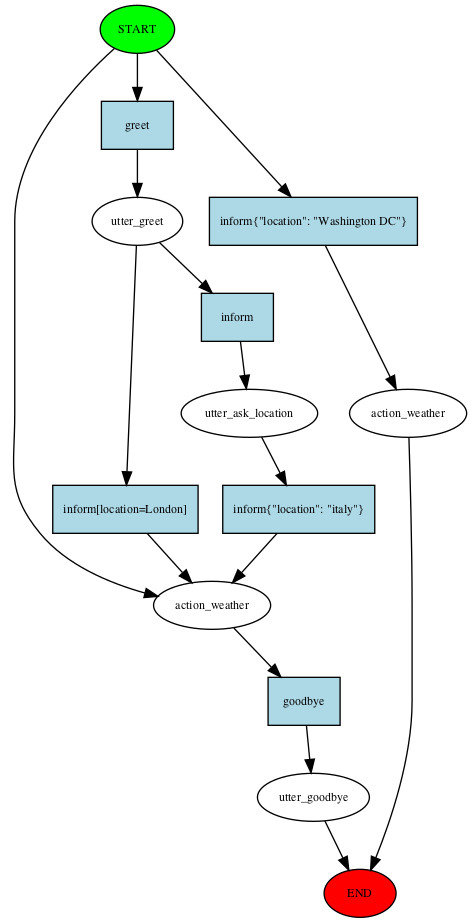
\includegraphics[width=0.5\linewidth,keepaspectratio]{graph1}
%   \caption{A \color{blue} directed \color{black} graph (digraph).}
    \end{figure}
    
(Ref: COMP26120 Manchester)
\end{frame}

%%%%%%%%%%%%%%%%%%%%%%%%%%%%%%%%%%%%%%%%%%%%%%%%%%%%%%%%%%%
   \begin{frame}[fragile]
    \begin{figure} [ht]
    \centering
    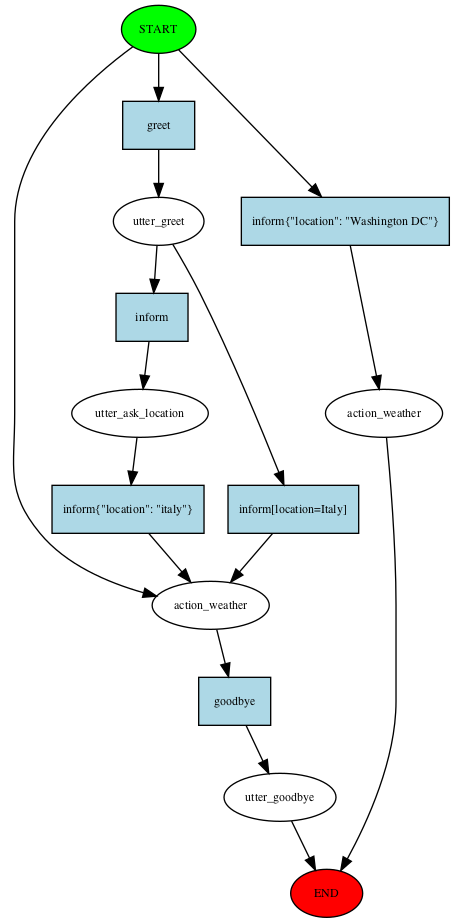
\includegraphics[width=0.7\linewidth,keepaspectratio]{graph2}
%    \caption{An \color{blue}undirected \color{black} graph (a \color{blue}multigraph \color{black} - more than one edge possible between pairs of nodes).}
    \end{figure}
\end{frame}

%%%%%%%%%%%%%%%%%%%%%%%%%%%%%%%%%%%%%%%%%%%%%%%%%%%%%%%%%%%
   \begin{frame}[fragile]
    \begin{figure} [ht]
    \centering
    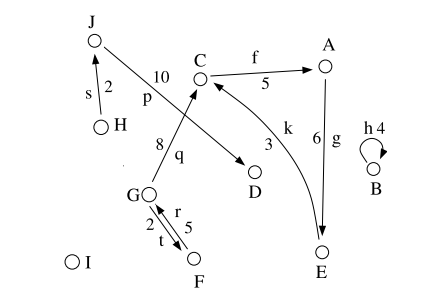
\includegraphics[width=0.7\linewidth,keepaspectratio]{graph3}
%    \caption{An \color{blue}edge-weighted \color{black} directed graph.}

    \end{figure}

\end{frame}
 
 %%%%%%%%%%%%%%%%%%%%%%%%%%%%%%%%%%%%%%%%%%%%%%%%%%%%%%%%%%%
   \begin{frame}[fragile]
\frametitle{Applications}

\begin{tabular}{lccc}
Application & Nodes & Edges & Type of graph \\
\hline \\
Wired Networks & Computers & Cables & Undirected multigraph \\
............................ & ................ & ............... & ..................................\\
............................ & ................ & ............... & ..................................\\
............................ & ................ & ............... & ..................................\\
............................ & ................ & ............... & ..................................\\
............................ & ................ & ............... & ..................................\\
............................ & ................ & ............... & ..................................\\
............................ & ................ & ............... & ..................................\\
............................ & ................ & ............... & ..................................\\
............................ & ................ & ............... & ..................................\\
............................ & ................ & ............... & ..................................\\
............................ & ................ & ............... & ..................................\\
............................ & ................ & ............... & ..................................
\end{tabular}

\end{frame}

%%%%%%%%%%%%%%%%%%%%%%%%%%%%%%%%%%%%%%%%%%%%%%%%%%%%%%%%%%%
   \begin{frame}[fragile]
\frametitle{Terminology}

\begin{itemize}
\item Nodes - sometimes called vertices, points, etc. 
\item Edges - sometimes called arcs, lines, etc.

\item Two nodes linked by an edge are \color{blue}adjacent \color{black} or, simply \color{blue}linked\color{black}.

\item For directed graphs, an edge $e$ from node $A$ to node $B$, is said to have $A$ as
its \color{blue}source \color{black} node (or start or origin node) and $B$ as its \color{blue}target \color{black} node (or end or finish or destination node).

\item An edge is  \color{blue}incident \color{black} on a node if it has the node as source or target (directed) or
if it links the node to another (undirected).

\item For an undirected graphs, the number of edges incident at a node is the  \color{blue}degree \color{black} of the node.
For directed graphs, the number of edges whose source is a node, is the  \color{blue}out-degree \color{black} of the node, likewise targets and  \color{blue}in-degree \color{black}.
\end{itemize}
\end{frame}

%%%%%%%%%%%%%%%%%%%%%%%%%%%%%%%%%%%%%%%%%%%%%%%%%%%%%%%%%%%
   \begin{frame}[fragile]
\frametitle{More terminology: Paths}

\begin{itemize}
\item A \color{blue}path \color{black} is a sequence (possibly empty) of adjacent nodes and the linking edges, in the case of undirected graphs. 

\item In the case of directed graphs, a \color{blue}path \color{black} is a sequence  (possibly empty) of adjacent nodes 
and linking edges, but with all edges in the same direction. 

\item If there is a path from node $A$ to node $B$, we say $B$ is \color{blue}reachable \color{black} from $A$.

\item A path from a node to itself is a \color{blue}cycle\color{black}.

\item A \color{blue}loop \color{black} is an edge from a node to itself.
\end{itemize}
\end{frame}

%%%%%%%%%%%%%%%%%%%%%%%%%%%%%%%%%%%%%%%%%%%%%%%%%%%%%%%%%%%
   \begin{frame}[fragile]
\frametitle{More terminology: Connected graphs}

\begin{itemize}
\item Two nodes in an undirected graph are \color{blue}connected \color{black} if there is a path between them. 

\item For directed graphs, the notion of `connected' is different (warning: the textbook doesn't make this clear):

\item Two nodes in a directed graph are \color{blue}connected \color{black} 
if there is a sequence of adjacent nodes between them. (Notice that the edges can be in any direction between nodes in the sequence.)

\item A graph is \color{blue}connected \color{black} if all pairs of nodes are connected.
\end{itemize}
\end{frame}

%%%%%%%%%%%%%%%%%%%%%%%%%%%%%%%%%%%%%%%%%%%%%%%%%%%%%%%%%%%
   \begin{frame}[fragile]
\frametitle{More terminology: Components}

\begin{itemize}
\item A \color{blue}subgraph \color{black} of a graph $G$, is a graph whose nodes and edges are a subset of those of 
$G$ and whose edges have the same source and target as those of $G$.

\item A \color{blue}connected component \color{black} (sometimes, just a `component') of a graph $G$, is a largest
connected subgraph (i.e.~one that cannot be expanded with additional nodes without 
becoming disconnected).

\item Every graph can be partitioned into disjoint connected components. 

\item \color{blue}Question\color{black}: How do we compute the components of a graph efficiently? Is there a quadratic algorithm O($N^2$) or even a linear algorithm O($N$), where $N$ is the number of nodes - what about the number of edges?
\end{itemize}

\end{frame}
%
%%%%%%%%%%%%%%%%%%%%%%%%%%%%%%%%%%%%%%%%%%%%%%%%%%%%%%%%%%%%
%   \begin{frame}[fragile]
%
%\begin{center}
%\frametitle{More about graphs}
%\end{center}
%More about graphs:
%\begin{itemize}
%\item representing graphs in programming languages,
%\item traversal techniques for trees and graphs.
%\end{itemize}
%
%This is material from Chapter 6  of \color{red}the course textbook\color{black}. 
%\end{frame}

%%%%%%%%%%%%%%%%%%%%%%%%%%%%%%%%%%%%%%%%%%%%%%%%%%%%%%%%%%%
   \begin{frame}[fragile]
\frametitle{Representing graphs}

\begin{itemize}
\item How do we represent graphs using the data types commonly provided in programming languages:
arrays, linked lists, vectors, 2-D arrays etc?

\item There are several representations in widespread use. We deal with the two commonest. 

\item Which to choose depends on
\begin{itemize}
\item properties of the graph (e.g.~`sparseness'), 
\item the algorithms we wish to implement, 
\item the programming language and how data structures are implemented, and
\item application of the code.
\end{itemize}
\end{itemize}
\end{frame}

%%%%%%%%%%%%%%%%%%%%%%%%%%%%%%%%%%%%%%%%%%%%%%%%%%%%%%%%%%%
   \begin{frame}[fragile]
\frametitle{Representing graphs: Adjacency lists}

An \color{blue}adjacency list \color{black} representation of a graph 
consists of a list of all nodes, and with each node
$n$ a list of all adjacent nodes (for directed graphs, these are the nodes 
that are the target of edges with source $n$).

  \begin{columns}
    \begin{column}{0.5\linewidth}
    
    \begin{figure} [ht]
    \centering
    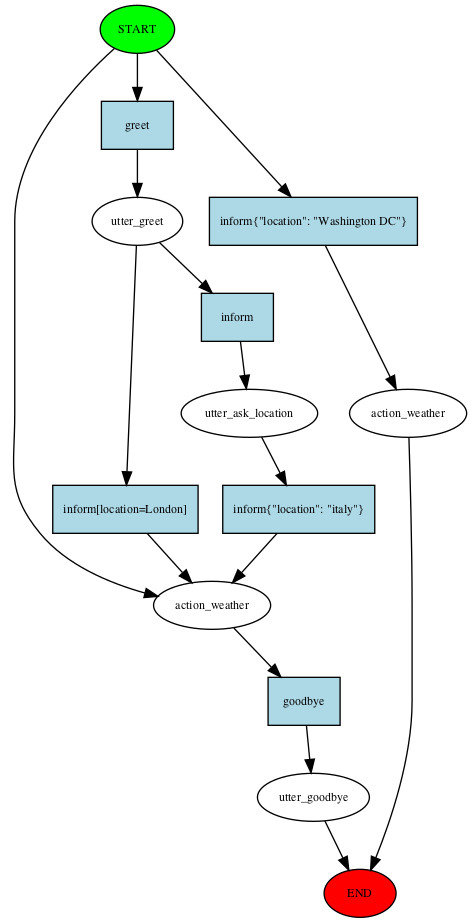
\includegraphics[width=0.9\linewidth,keepaspectratio]{graph1}
%    \caption{A \color{blue}directed \color{black} graph.}
    \end{figure}
	\end{column}
	    \begin{column}{0.5\linewidth}
	
{\scriptsize
\begin{tabular}{c|l}
Node & Adjacent nodes \\
\hline 
A & E\\
B & B \\
C & A \\
D & \\
E & C \\
F & G \\
G & F, C \\
H & J \\
I & \\
J & D 
\end{tabular}

}
	\end{column}
  \end{columns}
\end{frame}

%%%%%%%%%%%%%%%%%%%%%%%%%%%%%%%%%%%%%%%%%%%%%%%%%%%%%%%%%%%
   \begin{frame}[fragile]
\frametitle{Representing graphs: Adjacency matrices}

An \color{blue}adjacency matrix \color{black} representation of a graph consists of a 2-dimensional array (or matrix), each dimension indexed by the nodes of the graph. The entries in the matrix are:
\begin{itemize}
\item \color{red}1 \color{black} at index $(m,n)$ if there is an edge from $m$ to $n$,
\item \color{red}0 \color{black} at index $(m,n)$ if there is no edge from $m$ to $n$.
\end{itemize}

\end{frame}

%%%%%%%%%%%%%%%%%%%%%%%%%%%%%%%%%%%%%%%%%%%%%%%%%%%%%%%%%%%
   \begin{frame}[fragile]

  \begin{columns}
    \begin{column}{0.4\linewidth}
    

    \begin{figure} [ht]
    \centering
    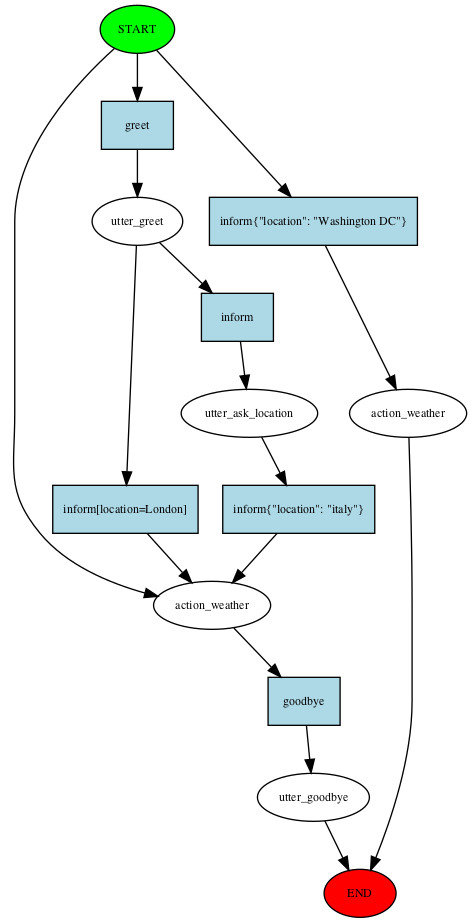
\includegraphics[width=0.9\linewidth,keepaspectratio]{graph1}
%    \caption{A \color{blue}directed \color{black} graph.}
    \end{figure}
	\end{column}
	    \begin{column}{0.6\linewidth}

{\scriptsize
   \begin{figure} [ht]
\begin{center}
\begin{tabular}{c|cccccccccc}
  & A & B & C & D & E & F & G & H & I & J \\
\hline 
A & 0 & 0 & 0 & 0 & 1 & 0 & 0 & 0 & 0 & 0 \\
B & 0 & 1 & 0 & 0 & 0 & 0 & 0 & 0 & 0 & 0 \\
C & 1 & 0 & 0 & 0 & 0 & 0 & 0 & 0 & 0 & 0 \\
D & 0 & 0 & 0 & 0 & 0 & 0 & 0 & 0 & 0 & 0 \\
E & 0 & 0 & 1 & 0 & 0 & 0 & 0 & 0 & 0 & 0 \\
F & 0 & 0 & 0 & 0 & 0 & 0 & 1 & 0 & 0 & 0 \\ 
G & 0 & 0 & 1 & 0 & 0 & 1 & 0 & 0 & 0 & 0 \\ 
H & 0 & 0 & 0 & 0 & 0 & 0 & 0 & 0 & 0 & 1 \\
I & 0 & 0 & 0 & 0 & 0 & 0 & 0 & 0 & 0 & 0 \\ 
J & 0 & 0 & 0 & 1 & 0 & 0 & 0 & 0 & 0 & 0   
\end{tabular}
\end{center}
%   \caption{Adjacency matrix representation of above graph (source nodes on the left)}
    \end{figure}
}
	\end{column}
  \end{columns}
\end{frame}

%%%%%%%%%%%%%%%%%%%%%%%%%%%%%%%%%%%%%%%%%%%%%%%%%%%%%%%%%%%
  \begin{frame}[fragile]
\frametitle{Representing graphs: Notes}

\begin{itemize}
\item These are both \color{blue}tabular \color{black} representations. The exact choice of types to represent them depends on the application. 

For example, an adjacency list may be an array of linked lists, if we wish to have fast 
(random) access to the lists of adjacent nodes, but to iterate through these lists.

\item Notice how  \color{blue}sparse \color{black} the adjacency matrix is: most entries are zero as there are few edges in the graph.

\end{itemize}

\end{frame}

%%%%%%%%%%%%%%%%%%%%%%%%%%%%%%%%%%%%%%%%%%%%%%%%%%%%%%%%%%%
   \begin{frame}[fragile]
\frametitle{Representing graphs: Notes}

\begin{itemize}

\item The representations need modification to include various data. For example, for a  \color{blue}multigraph\color{black}, we may record the edges as well as the adjacent nodes in a list representation, or the number of edges in a matrix representation. Also for  \color{blue}edge-weighted graphs, \color{black} we include the weights in the representation.

\item Notice that for undirected graphs, the matrix is  \color{blue}symmetrical\color{black}.
\end{itemize}

\end{frame}

%%%%%%%%%%%%%%%%%%%%%%%%%%%%%%%%%%%%%%%%%%%%%%%%%%%%%%%%%%%
  \begin{frame}[fragile]
\begin{itemize}
\item Adjacency matrices allow us to do  \color{blue}arithmetic\color{black}! We may add and multiply matrices, take determinants etc. These determine transformations of graphs and values derived from graphs.

\item \color{blue}Different representations for different tasks\color{black}: We choose which representation to use
by considering the efficiency of an algorithm for the task. 

\end{itemize}

\end{frame}

%%%%%%%%%%%%%%%%%%%%%%%%%%%%%%%%%%%%%%%%%%%%%%%%%%%%%%%%%%%
  \begin{frame}[fragile]

\color{blue}Example\color{black}: Consider the task of finding whether there is a path of length 2 from a given node
$S$ to another node $T$. For adjacency lists, we consider the list of nodes adjacent to
$S$ - in the worst case this is of length $E$ (the number of edges of the graph). For each node
in this list we see whether $T$ is in its list. Thus the worst-case time complexity is 
$E\times E$. Using adjacency matrices, this complexity is $N$ (the number of nodes) - why?

In general, for path finding algorithms, adjacency lists are sometimes more efficient, 
adjacency matrices for other algorithms.
\end{frame}

%%%%%%%%%%%%%%%%%%%%%%%%%%%%%%%%%%%%%%%%%%%%%%%%%%%%%%%%%%%
  \begin{frame}[fragile]
\frametitle{Traversals: Trees}

A traversal of a tree or graph is a means of visiting the nodes using the edges and
revisits of nodes. Usually, there are rules to determine possible next nodes to 
visit or revisit.

There are many techniques, the most widely used are \color{blue}Depth-First Search \color{black} and \color{blue}Breadth-First Search\color{black}.

For \color{red}trees\color{black}, we start at the root and: 

\begin{itemize}
\item For \color{blue}Depth-First Search \color{black} (DFS), visit all descendants of a node, before visiting sibling nodes;
\item For  \color{blue}Breadth-First Search \color{black} (BFS), visit all children of a node, then all grandchildren, etc;
\end {itemize}

\end{frame}

%%%%%%%%%%%%%%%%%%%%%%%%%%%%%%%%%%%%%%%%%%%%%%%%%%%%%%%%%%%
  \begin{frame}[fragile]
\frametitle{Traversals of trees: Examples}

  \begin{columns}
    \begin{column}{0.5\textwidth}

    \begin{figure} [ht]
    \centering
    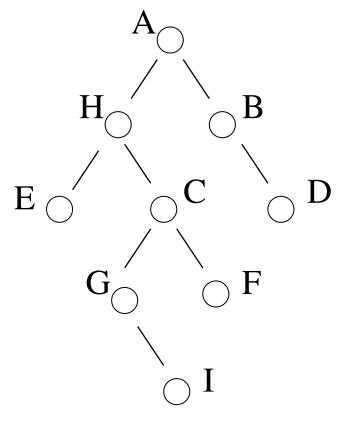
\includegraphics[width=0.8\linewidth,keepaspectratio]{tree_binary}
    \end{figure}
    \end{column}
    
        \begin{column}{0.5\textwidth}

\begin{enumerate}
\item A Depth-First Search from the root \color{blue}A \color{black} (in terms of order of visiting nodes): \color{blue}A,H,C,F,G,I,E,B,D.\color{black}
\item Another DFS (left-to-right): \color{blue}A,H,E,C,G,I,F,B,D.\color{black}
\item For DFS, the revisiting of nodes takes place through \color{red}backtracking\color{black}.
\item A Breadth-First Search (right-to-left): \color{blue}A,B,H,D,C,E,F,G,I.\color{black}
\end{enumerate}
    \end{column}
      \end{columns}
\end{frame}

%%%%%%%%%%%%%%%%%%%%%%%%%%%%%%%%%%%%%%%%%%%%%%%%%%%%%%%%%%%
  \begin{frame}[fragile]
\frametitle{Priority search}

Now let trees have a \color{blue}numerical priority\color{black}\ assigned to each node.

A \color{red}priority search\color{black}\ is:

\begin{enumerate}
\item Visit the root.
\item At each step, visit a node that has \color{blue}{highest priority}\ amongst unvisited children of visited nodes.
\end{enumerate}

Priority searches are often used to implement \color{blue}{heuristic search methods}\ where the priority is calculated at each node to provide an indication of whether a route through this node is likely to reach a required goal.

\end{frame}

%%%%%%%%%%%%%%%%%%%%%%%%%%%%%%%%%%%%%%%%%%%%%%%%%%%%%%%%%%%
  \begin{frame}[fragile]
\frametitle{Priority search: Example}

As an example consider the tree:

\begin{quote}
\begin{center}
\begin{figure} [ht]
    \centering
    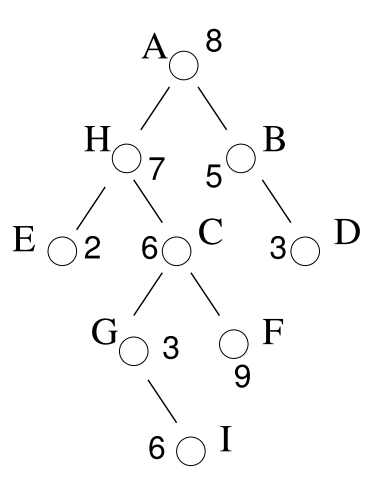
\includegraphics[width=0.5\linewidth,keepaspectratio]{priority-tree}
    \end{figure}
\end{center}
\end{quote}

One priority search of this tree is: A, H, C, F, B, G, I, D, E.
\end{frame}


%%%%%%%%%%%%%%%%%%%%%%%%%%%%%%%%%%%%%%%%%%%%%%%%%%%%%%%%%%%
  \begin{frame}[fragile]
\frametitle{Generic search routine for trees}

We now show how we can code \alert{all} the above search techniques (traversals) of tree \color{blue}with the same program\color{black}.

The program uses an auxiliary date structure with operations \color{blue}push, pop, top, empty\color{black}.

\begin{itemize}
\item When the data structure is a \alert{stack}\ the traversal is \color{blue}{DFS},
\item When the data structure is a \alert{queue}\ the traversal is \color{blue}{BFS},
\item When the data structure is a \alert{priority queue}\ the traversal is a \color{blue}{priority search}.
\end{itemize}

A \color{blue}{priority queue}\ has the operations of a queue (push, pop, top, empty), but top \color{blue}{returns an item of highest priority in the queue}\ and pop removes this item.
\end{frame}

%%%%%%%%%%%%%%%%%%%%%%%%%%%%%%%%%%%%%%%%%%%%%%%%%%%%%%%%%%%
  \begin{frame}[fragile]
\frametitle{Generic search routine for trees - program}

\color{red}{Idea}: 
\begin{enumerate}
\item Start by pushing root node of the tree onto the structure. 
\item Then visit the top element on the structure, pop it and push its children onto the structure.
\end{enumerate}

The structure therefore stores the unvisited children of visited nodes in the order in which they are encountered.
\end{frame}

%%%%%%%%%%%%%%%%%%%%%%%%%%%%%%%%%%%%%%%%%%%%%%%%%%%%%%%%%%%
  \begin{frame}[fragile]
\frametitle{Generic search routine for trees - pseudocode}

The pseudocode \color{blue}{labels each node u with search-num(u)}\ giving the order the nodes are encountered:

\begin{verbatim}
   u <- rootnode;
   s <- empty;
   i <-  0;
   push(u,s);
   while s not empty do
    { i <-  i+1;
      u <- top(s);
      search-num(u) <- i;
      pop(s);
      forall v children of u
        push(v,s) }
\end{verbatim}

Exercise: Hand run examples above.
\end{frame}

%%%%%%%%%%%%%%%%%%%%%%%%%%%%%%%%%%%%%%%%%%%%%%%%%%%%%%%%%%%
  \begin{frame}[fragile]
\frametitle{Traversals: From trees to graphs}

A tree is a directed graph such that:
\begin{quote}\color{blue}
There is a distinguished node (the root) such that there is a unique path from the root to any node in the graph.
\color{black}\end{quote}

To modify tree traversal for graphs:
\begin{enumerate}
\item We may revisit nodes: so mark nodes as visited/unvisited and only continue traversal from unvisited nodes.
\item There may not be one node from which all others are reachable: so choose node, perform traversal, then start traversal again from any unvisited nodes.
\end{enumerate}
\end{frame}


%%%%%%%%%%%%%%%%%%%%%%%%%%%%%%%%%%%%%%%%%%%%%%%%%%%%%%%%%%%
  \begin{frame}[fragile]
\frametitle{Traversals of Graphs: Examples}


    \begin{figure} [ht]
    \centering
    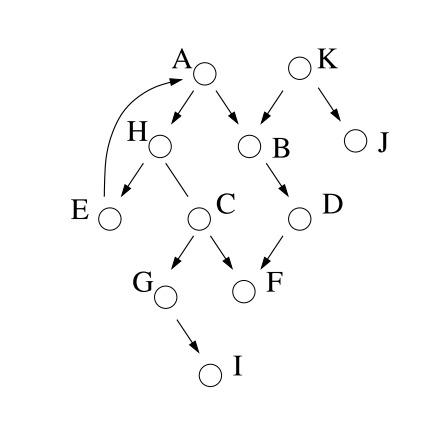
\includegraphics[width=0.5\linewidth,keepaspectratio]{graph5}
    \end{figure}

A Depth-First Search: \color{blue}A,H,E,C,F,G,I,B,D,K,J.\color{black}

A Breadth-First Search: \color{blue}A,H,B,E,C,D,G,F,I,K,J.\color{black}
\end{frame}

%%%%%%%%%%%%%%%%%%%%%%%%%%%%%%%%%%%%%%%%%%%%%%%%%%%%%%%%%%%
  \begin{frame}[fragile]
  \frametitle{Depth-First Search for Graphs: Recursive Algorithm}

Allocates a number \color{blue}dfsnum(u) \color{black} to each node u in a graph, giving the order of 
encountering nodes in a depth-first search on a graph. Notice how we use this numbering to 
determine whether or not we have visited a node before (Zero = No, Non-zero = Yes).

\begin{verbatim}
   forall nodes u do dfsnum(u) <- 0 end;
   i <- 0;

   visit(u) =
      { i <- i+1;
        dfsnum(u) <- i;
        forall nodes v adjacent to u do
          if dfsnum(v) = 0 then visit(v) end };

   forall nodes u do
      if dfsnum(u) = 0 then visit(u) end;
\end{verbatim}
\end{frame}

%%%%%%%%%%%%%%%%%%%%%%%%%%%%%%%%%%%%%%%%%%%%%%%%%%%%%%%%%%%
  \begin{frame}[fragile]\frametitle{The complexity of DFS}

For a graph with $N$ nodes and $E$ edges:
\begin{itemize}
\item For the \color{blue}adjacency list\color{black}\ representation, the complexity is linear $O(N+E)$,
\item For the \color{blue}adjacency matrix\color{black}\ representation, the complexity is quadratic $O(N^2)$.
\end {itemize}

\alert{Why?}
\end{frame}

%%%%%%%%%%%%%%%%%%%%%%%%%%%%%%%%%%%%%%%%%%%%%%%%%%%%%%%%%%%
  \begin{frame}[fragile]
\frametitle{Traversals of graphs: Notes}

\begin{itemize}
\item The actual order determined by a depth-first search is that of a \color{blue}stack-based discipline\color{black},
that is when we backtrack we visit the `most recent' unvisited branch first, 
before backtracking to more remote ancestors.

\item Breadth-First Search does not have such a recursive formulation. 

\item The \color{blue}{generic code for trees}\ above extends to graphs to provide DFS, BFS and priority search for graphs using the same auxiliary data structures.
\end{itemize}
\end{frame}

%%%%%%%%%%%%%%%%%%%%%%%%%%%%%%%%%%%%%%%%%%%%%%%%%%%%%%%%%%%
  \begin{frame}[fragile]\frametitle{Survey of graph algorithms}

\color{red}A brief overview of some topics in graph theory, looking at algorithms available\color{black}:

Many graph algorithms are based on the traversals:  \color{blue}DFS, BFS and Priority Search\color{black}. 

For example, there are efficient (usually linear) algorithms based on \color{blue}Depth-First Search\color{black}\ for:

\begin{itemize}
\item finding the connected components of a graph (how? - consider the case of undirected graphs),
\item detecting cycles in a graph,
\item finding `strong components' of a graph, 
\item planarity testing and embedding (see below), 
\item articulation points and blocks of undirected graphs, 
`orient-ability' and `reducibility' of graphs, etc.
\end{itemize}

\end{frame}

%%%%%%%%%%%%%%%%%%%%%%%%%%%%%%%%%%%%%%%%%%%%%%%%%%%%%%%%%%%
   \begin{frame}[fragile]\frametitle{Survey of graph algorithms: Path finding}

There are numerous \color{blue}path-finding problems\color{black}\ in graphs and a variety of algorithms:

\begin{itemize}
\item To find all paths between all pairs of nodes (`transitive closure'), or
\item To find all paths between a fixed pair of nodes, or
\item To find all paths from one node to all others (the `single source problem').
\end{itemize}

When the edges are labelled with numerical values, then we can ask for \color{blue}{shortest paths}\color{black},
by which we mean a path of minimum length, where the length of a path is the sum of 
its edge labels. 

Each problem above yields a shortest path problem - an example of an \color{blue}optimization problem\color{black}.

In fact, the second and third problems are equivalent.

\end{frame}

%%%%%%%%%%%%%%%%%%%%%%%%%%%%%%%%%%%%%%%%%%%%%%%%%%%%%%%%%%%
  \begin{frame}[fragile]\frametitle{Survey of graph algorithms: Path finding (continued)}

\begin{itemize}
\item There is an \alert{optimization property} concerning shortest paths:

\begin{quote}
If $p$ is a shortest path from node $u$ to node $v$ via node $w$, then the portions 
of $p$ from $u$ to $w$ and from $w$ to $v$ are both shortest paths.
\end{quote}

\item Proof: Evident!

\item Such optimization properties mean that there are direct methods of computing 
shortest paths: To accumulate shortest paths we need combine only other shortest paths 
(and not consider any other paths).

\item This is the basis of both \color{blue}Floyd's Algorithm\color{black}\ and \color{blue}Dijkstra's Algorithm\color{black}.
\end{itemize}
\end{frame}

%%%%%%%%%%%%%%%%%%%%%%%%%%%%%%%%%%%%%%%%%%%%%%%%%%%%%%%%%%%
  \begin{frame}[fragile]\frametitle{Survey of graph algorithms: Planarity}

\begin{itemize}
\item Planarity is about \color{blue}depicting graphs in 2-D space\color{black}: how do we `draw' graphs and 
can we do so without edges crossing.

\item \color{blue}{\bf Definition}\color{black}: An \alert{embedding} of a (directed or undirected) graph in the plane is an allocation of distinct points in the plane
to the nodes and distinct continuous lines (not necessarily straight - that is another problem) to the edges, so that no two lines intersect.

\item There may be more than one `way' of embedding a graph in the plane. \color{blue}Can all graphs be embedded in the plane?\color{black}\ \alert{No!}

\item A graph that can be embedded in the plane is called a \color{blue}{planar}\color{black}\ graph.

\item  Hopcroft and Tarjan introduced a \color{blue}linear-time planarity algorithm\color{black}\ (1974) based on Depth-First Search
\end{itemize}

\end{frame}

%%%%%%%%%%%%%%%%%%%%%%%%%%%%%%%%%%%%%%%%%%%%%%%%%%%%%%%%%%%
  \begin{frame}[fragile]
\frametitle{Two non-planar graphs:}

    \begin{figure} [ht]
    \centering
    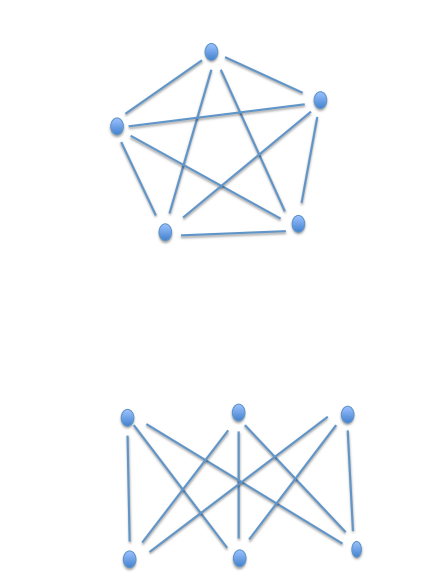
\includegraphics[width=0.5\linewidth,keepaspectratio]{nonplanar}
    \end{figure}


\end{frame}

%%%%%%%%%%%%%%%%%%%%%%%%%%%%%%%%%%%%%%%%%%%%%%%%%%%%%%%%%%%
  \begin{frame}[fragile]\frametitle{Survey of graph algorithms: Graph colouring}

\begin{itemize}
\item A \alert{colouring} of a graph with $k$ colours is an allocation of the colours to the nodes of the graph, such that each node has just one colour and nodes linked by an edge have different colours.

\item To determine whether a graph can be coloured with $k$ ($k\ge 3$) colours is 
an \alert{NP-complete problem}.

\item Thus the only algorithms that exist in general for colourability are exhaustive 
unlimited back-tracking algorithms, and hence are \color{blue}{exponential-time}\color{black}.
\end{itemize}
\end{frame}


%%%%%%%%%%%%%%%%%%%%%%%%%%%%%%%%%%%%%%%%%%%%%%%%%%%%%%%%%%%
  \begin{frame}[fragile]
\frametitle{Survey of graph algorithms: Finale}


The \color{blue}{4-colouring of planar graphs}\color{black}... is a \alert{celebrated problem}.

\color{blue}{\bf Proposition}\color{black}\ Every planar graph can be coloured with just 4 colours. 

\begin{itemize}
\item Discussed as a possibility in the 1850s,
\item 1879: Kempe publishes a `proof' of the 4-colour theorem,
\item 1890: Heawood finds error in Kempe's proof, but shows Kempe's proof establishes the 5-colourability of planar graphs,
\item Since then finding a proof of 4-colourability has been a catalyst for much combinatorial mathematics,
\item 1977: Computer-aided proof of 4-colourability: reduced the graphs required to be coloured to a finite number (over 1000) and then used a computer to generate colourings.
\end{itemize}
\end{frame}


%%%%%%%%%%%%%%%%%%%%%%%%%%%%%%%%%%%%%%%%%%%%%%%%%%%%%%%%%%%
   \begin{frame}[fragile]{Shortest Path}

  \begin{itemize}
  \item Computational finance: 
    \begin{itemize}
    \item Each node is a financial agent.
    \item The cost $c_{uv}$ of an edge $(u, v)$ is the cost of a
      transaction in which we buy from agent $u$ and sell to agent $v$.
    \item Negative cost corresponds to a profit.
    \end{itemize}
  \item Internet routing protocols
    \begin{itemize}
    \item Dijkstra's algorithm needs knowledge of the entire network.
    \item Routers only know which other routers they are connected to.
    \item Algorithm for shortest paths with negative edges is decentralized.
    \item We will not study this algorithm in the class. See Chapter 6.9.
    \end{itemize} 
  \end{itemize} 
\end{frame}

%%%%%%%%%%%%%%%%%%%%%%%%%%%%%%%%%%%%%%%%%%%%%%%%%%%%%%%%%%%
   \begin{frame}[fragile]{Problem Statement} 

  \begin{itemize}
  \item Input: a directed graph $G = (V, E)$ with a cost function $c: E
    \rightarrow $, i.e., $c_{uv}$ is the cost of the edge $(u, v)
    \in E$.
  \item A \textbf{negative cycle} is a directed cycle whose edges have a
    total cost that is negative.
  \item Two related problems:
    \begin{enumerate}
    \item If $G$ has no negative cycles, find the \textbf{shortest
        $s$-$t$ path}: a path of from source $s$ to destination $t$ with
      minimum total cost.
    \item Does $G$ have a \textbf{negative cycle}?
    \end{enumerate}
  \end{itemize}
   

\end{frame}

%%%%%%%%%%%%%%%%%%%%%%%%%%%%%%%%%%%%%%%%%%%%%%%%%%%%%%%%%%%
   \begin{frame}[fragile]{Approaches for Shortest Path Algorithm}

  \begin{columns}
    \begin{column}{0.5\textwidth}
      \begin{enumerate}
      \item Dijsktra's algorithm. {Computes incorrect
          answers because it is greedy.}
      \item Add some large constant to each edge.
        {Computes incorrect answers because the minimum
          cost path changes.}
      \end{enumerate}
    \end{column}
    
    \begin{column}{0.5\textwidth}
      {
 \begin{center}
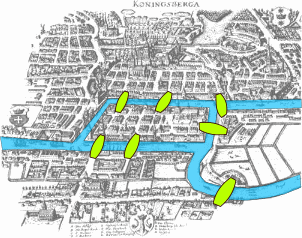
\includegraphics[width=\linewidth,keepaspectratio]{Konigsberg_bridges}
\end{center}
      }
    \end{column}
  \end{columns}
\end{frame}



%%%%%%%%%%%%%%%%%%%%%%%%%%%%%%%%%%%%%%%%%%%%%%%%%%%%%%%%%%%
   \begin{frame}[fragile]{Dynamic Programming Approach}

  \begin{itemize}
  \item Assume $G$ has no negative cycles.
  \item Claim: There is a shortest path from $s$ to $t$ that is
    \textbf{simple} (does not repeat a node)   and hence has at most $n -
    1$ edges.  
  \end{itemize}

\end{frame}


%%%%%%%%%%%%%%%%%%%%%%%%%%%%%%%%%%%%%%%%%%%%%%%%%%%%%%%%%%%
   \begin{frame}[fragile]{Dynamic Programming Approach}

      \begin{itemize}
      \item How do we define sub-problems?  

        \begin{itemize}
        \item Shortest $s$-$t$ path has $\leq n - 1$ edges: how we can
          reach $t$ using $i$ edges, for different values of $i$?
        \item We do not know which nodes will be in shortest
          $s$-$t$ path: how we can reach $t$ from each
          node in $V$? 
        \end{itemize}
      \item Sub-problems defined by varying the number of edges in the
        shortest path and by varying the starting node in the shortest
        path.
      \end{itemize}

\end{frame}

%%%%%%%%%%%%%%%%%%%%%%%%%%%%%%%%%%%%%%%%%%%%%%%%%%%%%%%%%%%
   \begin{frame}[fragile]{Dynamic Programming Recursion}

  \begin{itemize}
  \item \textbf{{i, v}}: minimum cost of a $v$-$t$ path that uses \alert{at
      most} $i$ edges.
  \item $t$ is not explicitly mentioned in the sub-problems.
  \item Goal is to compute {n - 1, s}.
     
  \end{itemize}

  \begin{itemize}
  \item Let $P$ be the optimal path whose cost is {i, v}. 
    \begin{enumerate}
    \item If $P$ actually uses $i - 1$ edges, then ${i, v} = {i - 1, v}$.
    \item If first node on $P$ is $w$, then ${i, v} = c_{vw} +
      {i - 1, w}$.
    \end{enumerate}
  \end{itemize}
   
  $${i, v} = \min \bigg( {i - 1, v}, \min_{w \in V} \big(c_{vw} +
      {i - 1, w} \big) \bigg)$$
\end{frame}

%%%%%%%%%%%%%%%%%%%%%%%%%%%%%%%%%%%%%%%%%%%%%%%%%%%%%%%%%%%
   \begin{frame}[fragile]{Alternate Dynamic Programming Formulation}

  \begin{itemize}
  \item \textbf{{i, v}}: minimum cost of a $v$-$t$ path that uses
    \alert{exactly} $i$ edges. Goal is to compute 
     
    $$ \min_{i=1}^{n-1}   {i, s}.$$
     
  \end{itemize}
%   \centerline{         
%     {\includegraphics[width=0.7\textwidth]{figs/extracted-figs/kleinberg-06-074}}%
%   }  
  \begin{itemize}
  \item Let $P$ be the optimal path whose cost is {i, v}. 
    \begin{itemize}
%     \item If $P$ uses $i - 1$ edges, then ${i, v} = {i - 1, v}$.
    \item If first node on $P$ is $w$, then ${i, v} = c_{vw} +
      {i - 1, w}$.
    \end{itemize}
  \end{itemize}
   
  $${i, v} = \min_{w \in V} \big(c_{vw} +
  {i - 1, w} \big) $$
   
  \begin{itemize}
  \item Compare the recurrence above to the previous recurrence:
  \end{itemize}
  $${i, v} = \min \bigg( {i - 1, v}, \min_{w \in V} \big(c_{vw} +
  {i - 1, w} \big) \bigg)$$
\end{frame}


%%%%%%%%%%%%%%%%%%%%%%%%%%%%%%%%%%%%%%%%%%%%%%%%%%%%%%%%%%%
   \begin{frame}[fragile]{Dijkstra's Algorithm}
\begin{enumerate}
\item Mark the ending vertex with a distance of zero.  Designate this vertex as current.
\item Find all vertices leading to the current vertex.  Calculate their distances to the end.  
Since we already know the distance the current vertex is from the end, this will just 
require adding the most recent edge.  Don't record this distance if it is longer than a 
previously recorded distance.
\item Mark the current vertex as visited.  We will never look at this vertex again.
\item Mark the vertex with the smallest distance as current, and re
peat from step 2.
\end{enumerate}
\end{frame}

%%%%%%%%%%%%%%%%%%%%%%%%%%%%%%%%%%%%%%%%%%%%%%%%%%%%%%%%%%%
   \begin{frame}[fragile]
Find the shortest path from $a$ to $g$.

% \tikzstyle{vertex}=[circle,fill=black!25,minimum size=20pt,inner sep=0pt]
% \tikzstyle{selected vertex} = [vertex, fill=red!24]
% \tikzstyle{edge} = [draw,thick,-]
% \tikzstyle{weight} = [font=\small]
% \tikzstyle{selected edge} = [draw,line width=5pt,-,red!50]
% \tikzstyle{ignored edge} = [draw,line width=5pt,-,black!20]


% \begin{figure}
% \begin{tikzpicture}[scale=1.8, auto,swap]
    % % Draw a 7,11 network
    % % First we draw the vertices
    % \foreach \pos/\name in {{(0,2)/a}, {(2,1)/b}, {(4,1)/c},
                            % {(0,0)/d}, {(3,0)/e}, {(2,-1)/f}, {(4,-1)/g}}
        % \node[vertex] (\name) at \pos {$\name$};
    % % Connect vertices with edges and draw weights
    % \foreach \source/ \dest /\weight in {b/a/7, c/b/8,d/a/5,d/b/9,
                                         % e/b/7, e/c/5,e/d/15,
                                         % f/d/6,f/e/8,
                                         % g/e/9,g/f/11}
        % \path[edge] (\source) -- node[weight] {$\weight$} (\dest);
        % %
% \end{tikzpicture}
% \end{figure}
\end{frame}


  \begin{frame}[fragile]
  \frametitle{Topics}
  
  Weighted graphs
  \begin{itemize} 
  \item each edge $(u,v)$ has a weight denoted $w(u,v)$ or $w_{uv}$
  \item stored in the adjacency list or adjacency matrix 
  \end{itemize} 
  
 
  The weight of a path $p= (v_1, v_2, v_3, ...v_k)$ is the sum of the weights of the edges on the path.
 
  Problems: 
  \begin{itemize}
  \item shortest paths (SP)
  \item minimum spanning tree (MST)
  \end{itemize}
\end{frame} 




  \begin{frame}[fragile]
  \frametitle{Shortest paths}
  Variants: 
  \begin{itemize} 
  \item P2P SP: given two vertices $u,v$: find SP from $u$ to $v$ 
  \item SSSP: given a vertex $u$, find SP from $u$ to all vertices  in $G$
  \item APSP: find SP between any two vertices $(u,v)$
  \end{itemize} 
  

Notes: 
\begin{itemize} 
\item SPs not well-defined when graph has a negative cycle
  \begin{itemize}
  \item might want shortest path that has no cycles $\Leftarrow$  NPC
  \end{itemize} 
  
\item When all edge weights are equal, SP can be computed by BFS.
  \begin{itemize}
  \item computing shortest paths in terms of number of edges on the path is a special case of the SP problem
  \end{itemize} 
  \end{itemize} 
\end{frame} 





  \begin{frame}[fragile]
  \frametitle{Point-to-point SP}

  Problem:   given two vertices $u,v$: find SP from $u$ to $v$ 


  No algorithm is known for computing SP(u,v) that's better, in the
  worst case, than running SSSP(u).
\end{frame} 



  \begin{frame}[fragile]
  \frametitle{APSP}

  Problem:   For any $u,v$: find SP from $u$ to $v$ 


Can run SSSP(u) $|V|$ times, once  for each vertex $u$. 
~\\~\\
Better algorithms exist. 
\end{frame} 



  \begin{frame}[fragile]
  \frametitle{SSSP}

  $G$ is a weighted (directed or undirected) graph. \\
  Problem: Given vertex $s$, find SP from $s$ to all $v$ in $G$.  

  
  If $G$ has positive weights: Diskstra's algorithm 

  Otherwise: Bellman-Ford algorithm 
\end{frame}



  \begin{frame}[fragile]
  \frametitle{SSSP: Dijkstra'a algorithm}
SSSP(s)\\
Idea: for each vertex $v$, maintain $d[v]$ as the best known shortest path to $v$ (from $s$)\\
~\\
Initially: $d[s]=0$ and  $d[v] = \infty$ for all $v \neq s$\\
~\\
Idea:  Greedy: Visit first the vertex with smallest $d$.  ~\\
~\\
Implementation: use a priority queue. \\
%With a heap, runs in $O(E \lg V)$
\end{frame}


  \begin{frame}[fragile]
  \frametitle{SSSP: Dijkstra'a algorithm}

\textcolor{blue}{Idea: for each vertex $v$, maintain $d[v]$ as the best known shortest path to $v$ (from $s$)}

 
\begin{itemize} 
\item  Initialize: $d[s]=0$ and  $d[v] = \infty$ for all $v \neq s$. For every $v \in V$, insert $(v,d[v])$ in PQ. 

\item while PQ not empty 
  \begin{itemize}
  \item $v  = $ deleteMin(PQ) 
  \item for each outgoing edge $(v,u)$: relax $(v,u)$
  \end{itemize} 
\end{itemize} 


relax$(v,u)$ tests whether we can improve the SP to $u$ by going through $v$
\begin{itemize} 
\item if $d[u] > d[v]+w_{vu}$ then 
  \begin{itemize}
  \item $d[u] = d[v]+w_{vu}$ 
  \item decreaseKey of $u$ in PQ to $d[u]$
  \end{itemize} 
\end{itemize} 

\textcolor{red}{$O(|V|+|E|) + |V| \cdot$ PQ-insert + $|V| \cdot $ PQ-delete + $|E| \cdot $ PQ-decreaseKey}
%With a heap, runs in $O(E \lg V)$
\end{frame}



  \begin{frame}[fragile]
  \frametitle{SSSP: Dijkstra'a algorithm}

\textcolor{blue}{Idea: for each vertex $v$, maintain $d[v]$ as the best known shortest path to $v$ (from $s$)}

 
\begin{itemize} 
\item  Initialize: $d[s]=0$ and  $d[v] = \infty$ for all $v \neq s$. For every $v \in V$, insert $(v,d[v])$ in PQ. 

\item while PQ not empty 
  \begin{itemize}
  \item $v  = $ deleteMin(PQ) 
  \item for each outgoing edge $(v,u)$: relax $(v,u)$
  \end{itemize} 
\end{itemize} 


relax$(v,u)$
\begin{itemize} 
\item if $d[u] > d[v]+w_{vu}$ then 
  \begin{itemize}
  \item $d[u] = d[v]+w_{vu}$ 
  \item decreaseKey of $u$ in PQ to $d[u]$
  \end{itemize} 
\end{itemize} 
\textcolor{red}{Analysis:   With a heap, runs in $O(E \lg V)$}
\end{frame}




  \begin{frame}[fragile]
  \frametitle{SSSP: Dijkstra'a algorithm}
Let $S$ denote the set of vertices that have been deleted from PQ. \\
Correctness: At every iteration of the \texttt{while} loop, the following invariants hold: 
\\
\begin{enumerate} 
\item \textcolor{blue}{(I1) for any $v \in V-S$, $d[v]$ is the length of the shortest
  path from $s$ to $v$ among all paths that go only through vertices
  of $S$.}
\item \textcolor{blue} {(I2) for any $v \in S$, $d[v]$ is the length of the shortest path from $s$ to $v$. }
\end{enumerate}

Prove by induction on the size of $S$. 
\end{frame} 



  \begin{frame}[fragile]
  \frametitle{SSSP: Dijkstra'a algorithm}
At every iteration of the \texttt{while} loop, the following holds: \\
\textcolor{blue}{(I1) for any $v \in V-S$, $d[v]$ is the length of the shortest
  path from $s$ to $v$ among all paths that go only through vertices
  of $S$.}

 
Basecase: (I1) is trivially true before the first iteration of the
while loop, when $S$ is empty.

Assume (I1) is true \emph{before} an iteration of the while loop.
We'll prove that it's true \emph{after} this iteration.
 
After adding $v$ to $S$, the only paths that can change are to those
vertices that are adjacent to $v$. The algorithm checks them and
releases them.
\end{frame} 





  \begin{frame}[fragile]
  \frametitle{SSSP: Dijkstra'a algorithm}
At every iteration of the \texttt{while} loop, the following holds: \\
\textcolor{blue} {(I2) for any $v \in S$, $d[v]$ is the length of the shortest path from $s$ to $v$. }
 
Basecase: (I2) is trivially true before the first iteration of the
while loop, when $S$ is empty.

Assume (I2) is true \emph{before} an iteration of the while loop.
We'll prove that it's true \emph{after} this iteration.
 

As we are adding $v$ to $S$, assume by contradiction that the length
of the shortest path to $v$ is $|\delta(s,v)| < d[v]$.  Let $(x,y)$ be the
first edge on $\delta(s,v)$ leaving $S$ ($x$ last vertex in $S$).

\begin{itemize} 
\item $d[v] > \delta(s,v) = \delta(s,y) + \delta(y,v)$
\item $d[y] = \delta(s,y)$  by (I1)
\item $d[v] < d[y]$ because $v$ comes out of PQ before $y$
\end{itemize}
$\Rightarrow \delta(y,v) < 0$ impossible
\end{frame} 



  \begin{frame}[fragile]
  \frametitle{SSSP: Dijkstra'a algorithm}

What happens if we run Dijkstra's algorithm on a graph with negative weights? 



Find an example of a graph where Dijkstra does not compute the SP correctly.



\end{frame} 


  \begin{frame}[fragile]
  \frametitle{SSSP with negative weights}
Note: If $G$ is undirected and has negative weights, that immediately means a negative cycle. 
  \end{frame}


  \begin{frame}[fragile]
  \frametitle{SSSP with negative weights}
  $G$ {\bf directed} graph. \\
   If $G$ has no negative cycles, then there exists a SP from
  $s$ to $v$ that is \emph{simple} and hence has $|V|-1$ edges.
   
  Let $\delta(u,v)$ denote the shortest path from $u$ to $v$. \\
  Start with $d[v] = \infty$ and progresively refine it, until $d[v] = |\delta(s,v)|$\\
  Similar to Dijkstra:  Dijkstra relaxes edges in greedy order of increasing $d[]$; that does
  not work for negative edges
 \end{frame} 


  \begin{frame}[fragile]
  \frametitle{SSSP with negative weights}
  $G$ {\bf directed} graph. \\
\alert{
  Bellman-Ford algorithm ($s$): \\
  \begin{itemize} 
  \item Initialize: $d[s]=0$ and $d[v] = \infty$ for all $v \neq
    s$. 
  \item for $i=1$ to $|V|-1$ do: 
    \begin{itemize}
    \item for every edge $(v,u)$ in $G$: relax$(v,u)$
    \end{itemize} 
  \end{itemize} 
}
  
  relax$(v,u)$
  \begin{itemize} 
  \item if $d[u] > d[v]+w_{vu}$ then 
    \begin{itemize}
    \item $d[u] = d[v]+w_{vu}$ 
    \end{itemize} 
  \end{itemize} 
\end{frame} 



  \begin{frame}[fragile]
  \frametitle{Bellman-Ford}
WHY does this work?\\
Intuition:  look at the number of edges along a shortest path (SP) from $s$
 
\begin{itemize} 
\item initially, only $d[s]$ is correct. Put differently, all SP that consist of  $0$ edges are correctly computed.
 
\item after round 1: all SP from $s$ that consist precisely of $1$ edge are correctly computed. 
 
\item after round 2: all SP from $s$ that consist precisely of $2$ edges are correctly computed. 

\item ...
\item after round $i$: all SP from $s$ that consist precisely of $i$ edges are correctly computed. 
\end{itemize} 
\end{frame} 



  \begin{frame}[fragile]
  \frametitle{Bellman-Ford}
WHY does this work?\\
Intuition:  look at the number of edges along a shortest path (SP) from $s$

\textcolor{gray}{Let $\delta(u,v)$ denote the shortest path from $u$ to $v$.}\\
\textcolor{blue}{Let $OPT(v,i)$ denote the length of the shortest path from $s$ to $v$ among all paths containing $\le i$ edges.} \\
 We have:
\begin{itemize} 

\item $OPT(s,0) = 0$

\item $OPT(v,0) = \infty$ for any $v \neq s$

\item $OPT(v, |V|-1) = |\delta(s,v)|$

\item $OPT(v,i) = min \{OPT(v, i-1), min_{u | (u,v)} \{ OPT(u,i-1) + w_{uv}\} \}$
\end{itemize} 

\textcolor{blue}{ Claim: After round $i$ in Bellman-Ford we have $d[v] = OPT(v,i)$}
\end{frame} 




  \begin{frame}[fragile]
  \frametitle{Bellman-Ford}

Running time:   $O(V\cdot E)$\\

After $V-1$ rounds, $d[v] = OPT(v, |V|-1) = |\delta(s,v)|$


What happens if we do more rounds? (beyond $|V|-1$)

\begin{itemize} 
\item the values $d[v]$ will not decrease any further.... unless.....there's a negative cycle
\end{itemize} 

 
Negative cycles:   What happens if $G$ negative cycles? 

\begin{itemize} 
\item $d[v]$ are not SP (there are no SP)
\item some values $d[v]$ will keep decreasing 
\end{itemize}


$\rightarrow$ Bellman-Ford can be used to test for the existence of negative cycles in the graph:
\end{frame} 




  \begin{frame}[fragile]
  \frametitle{Bellman-Ford}
  $G$ {\bf directed} graph. \\

  Bellman-Ford algorithm ($s$): \\
  \begin{itemize} 
  \item Initialize: $d[s]=0$ and $d[v] = \infty$ for all $v \neq
    s$. 
  \item for $i=1$ to $|V|-1$ do: 
    \begin{itemize}
    \item for every edge $(v,u)$ in $G$: relax$(v,u)$
    \end{itemize} 
  \item \textcolor{blue}{for each edge $(v,u)$ in $G$: if $d[v]+ w_{vu} < d[u] \Rightarrow$ NEG CYCLE  }
  \end{itemize} 


Note: detects negative cycle \emph{reachable from $s$}. Can be extended to detect if $G$ has any negative cycle. 
\end{frame} 



  \begin{frame}[fragile]
  \frametitle{SSSP}
  Summary of known algorithms: 
\textcolor{blue}  {
  \begin{itemize} 
  \item $G$ unweighted
    \begin{itemize} 
    \item BFS in $O(V+E)$
    \end{itemize} 
  \item $G$ DAG
    \begin{itemize} 
    \item   dynamic programming in $O(V+E)$
    \end{itemize} 
    \item $G$ directed, no negative weights
      \begin{itemize} 
      \item Dijkstra's algorithm in $O(E \lg V)$
      \end{itemize} 
    \item $G$ directed, no negative cycles
      \begin{itemize} 
        \item Bellman-Ford algorithm in $O(V\cdot E)$
        \end{itemize}
    \end{itemize} 
} 
\end{frame}

%%%%%%%%%%%%%%%%%%%%%%%%%%%%%%%%%%%%%%%%%%%%%%%%%%%%%%%%%%%%%%%%%%%%%%%%%%%%%%%%%%
   \begin{frame}[fragile]\frametitle{}
\begin{center}
{\Large Networks and Flows}

 - Vince Vatter

\end{center}
\end{frame}


%%%%%%%%%%%%%%%%%%%%%%%%%%%%%%%%%%%%%%%%%%%%%%%%%%%%%%%%%%%
\begin{frame}[fragile]{Networks and Flows}
   
Now we are going to think of our edges as pipes of varying sizes and our vertices as places where the pipes run together and the material we are piping can change direction.  Since pipes either flow one way or the other, we will be working with digraphs.  To model the fact that the pipes can be different sizes, we will assign a {\it capacity\/} to each arc, which we will write next to the arc.  We also have a {\it source\/}, which is where the things are being pumped from, and a {\it sink\/}, which is where the things are being pumped to.  I will always label the source $1$ and give the greatest label to the sink.  What we get when we do this is called a {\it network\/}.  Figure 6 shows a network.

\begin{center}
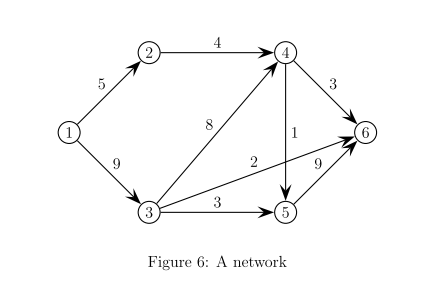
\includegraphics[width=0.5\linewidth,keepaspectratio]{vgraph1}
\end{center}

%\begin{figure}
%\begin{center}
%\begin{tabular}{c}
%
%\psset{arrows=->, arrowsize=9pt, labelsep=3pt, mnode=circle}
%\begin{psmatrix}
%&2&&4&[mnode=none] \\
%1&&&&6\\
%&3&&5&[mnode=none]
%\ncline{2,1}{1,2}\naput{5}
%\ncline{2,1}{3,2}\naput{9}
%\ncline{1,2}{1,4}\naput{4}
%\ncline{3,2}{3,4}\naput{3}
%\ncline{3,2}{1,4}\naput{8}
%\ncline{3,2}{2,5}\naput{2}
%\ncline{1,4}{3,4}\naput{1}
%\ncline{1,4}{2,5}\naput{3}
%\ncline{3,4}{2,5}\naput{9}
%\end{psmatrix}
%
%\end{tabular}
%\label{GexFlow}
%
%\end{center}
%\caption{A network}
%\end{figure}

\end{frame}
%%%%%%%%%%%%%%%%%%%%%%%%%%%%%%%%%%%%%%%%%%%%%%%%%%%%%%%%%%%
\begin{frame}[fragile]{Networks and Flows}


Let us give the various arc capacities names before going on:
$$
c_{i,j}
=
\mbox{the capacity of the arc from vertex $i$ to vertex $j$ ($0$ if there is no such arc).}
$$

We could put these into a matrix if we wanted.  Below is the capacity matrix for the graph in Figure 6.
$$
\left[\begin{array}{rrrrrr}
0&5&9&0&0&0\\
0&0&0&4&0&0\\
0&0&0&8&3&2\\
0&0&0&0&1&3\\
0&0&0&0&0&9\\
0&0&0&0&0&0
\end{array}
\right]
$$

\end{frame}
%%%%%%%%%%%%%%%%%%%%%%%%%%%%%%%%%%%%%%%%%%%%%%%%%%%%%%%%%%%
\begin{frame}[fragile]{Networks and Flows}


We want to figure out how to pump the maximum amount possible from the source to the sink.  In doing so we will construct a {\it flow\/}.  A flow will tell each pipe how much stuff to, well, pipe.  So a flow will be specified by a set of numbers $x_{i,j}$ which tell how much stuff the pipe from $i$ to $j$ will pipe.  (Like the $c_{i,j}$s, we will have $x_{i,j}=0$ if there is no arc from $i$ to $j$.)

Flows have to satisfy several restrictions.  First, a flow can't have a pipe piping more than it can pipe, so we will insist that
\begin{eqnarray}\label{flow1}
x_{i,j}&\le&c_{i,j}\mbox{ for all valid $i$ and $j$.}
\end{eqnarray}

But we're getting ahead of ourselves.  The first constraint we should have noticed is that pipes can't pipe negative amounts:
\begin{eqnarray}\label{flow2}
x_{i,j}&\ge&0\mbox{ for all valid $i$ and $j$.}
\end{eqnarray}

\end{frame}
%%%%%%%%%%%%%%%%%%%%%%%%%%%%%%%%%%%%%%%%%%%%%%%%%%%%%%%%%%%
\begin{frame}[fragile]{Networks and Flows}


The third and final constraint is known as Kirchkoff's Law.  It says that the amount flowing into a vertex must equal the amount flowing out of the vertex (unless that vertex is the source or the sink).  This comes from the fact that our vertices are just intersections, and don't have any storage capacity of their own.  The amount flowing out of vertex $i$ is given by
$$
\sum_{k=1}^n x_{i,k},
$$
where $n$ is the number of vertices in our network, and the amount flowing into vertex $i$ is given by
$$
\sum_{k=1}^n x_{k,i}.
$$
So in mathematical terms Kirchkoff's Law says
\begin{eqnarray}\label{flow3}
\sum_{k=1}^n x_{i,k}&=&\sum_{k=1}^n x_{k,i}\mbox{ for all valid $i$ except for the source and the sink.}
\end{eqnarray}

\end{frame}
%%%%%%%%%%%%%%%%%%%%%%%%%%%%%%%%%%%%%%%%%%%%%%%%%%%%%%%%%%%
\begin{frame}[fragile]{Networks and Flows}


That's it for the constraints.  What about the objective function?  We want to maximize the amount of stuff that gets pumped from the source to the sink.  Because of Kirchkoff's Law, everything that leaves the source must eventually get to the sink, so the amount of stuff that gets pumped from the source to the sink is
$$
\sum_{k=1}^n x_{1,k}.
$$
(Here we are using our convention that the source is vertex $1$.)  By Kirchkoff's Law again, this is the same as the amount of stuff that enters the sink:
$$
\sum_{k=1}^n x_{k,n}.
$$
(And here we are using our convention that the sink is vertex $n$.)

\end{frame}
%%%%%%%%%%%%%%%%%%%%%%%%%%%%%%%%%%%%%%%%%%%%%%%%%%%%%%%%%%%
\begin{frame}[fragile]{Networks and Flows}


Putting this, (\ref{flow1}), (\ref{flow2}), and (\ref{flow3}) together, we can write the problem as a linear programming problem.

$$
\begin{array}{l}
\mbox{Maximize $z=\sum_{k=1}^n x_{1,k}$}\\
\mbox{subject to}\\
\begin{array}{rcl}
\sum_{k=1}^n x_{i,k}&=&\sum_{k=1}^n x_{k,i}\mbox{ for all $i$ between $2$ and $n-1$}\\
x_{i,j}&\le&c_{i,j}\mbox{ for all $i$ and $j$ between $1$ and $n$}\\
x_{i,j}&\ge&0\mbox{ for all $i$ and $j$ between $1$ and $n$}
\end{array}
\end{array}
$$

\end{frame}
%%%%%%%%%%%%%%%%%%%%%%%%%%%%%%%%%%%%%%%%%%%%%%%%%%%%%%%%%%%
\begin{frame}[fragile]{Networks and Flows}

Since we usually like to get all our variables on the left-hand side, we can rewrite this as
$$
\begin{array}{l}
\mbox{Maximize $z=\sum_{k=1}^n x_{1,k}$}\\
\mbox{subject to}\\
\begin{array}{rcl}
\sum_{k=1}^n x_{i,k}-\sum_{k=1}^n x_{k,i}&=&0\mbox{ for all $i$ between $2$ and $n-1$}\\
x_{i,j}&\le&c_{i,j}\mbox{ for all $i$ and $j$ between $1$ and $n$}\\
x_{i,j}&\ge&0\mbox{ for all $i$ and $j$ between $1$ and $n$}
\end{array}
\end{array}
$$

Now we just have to solve this!  But, there are $n^2$ variables and $2n^2+n$ constraints, so the Simplex Method might not be the way to go.  Instead, we will use the...

\end{frame}
%%%%%%%%%%%%%%%%%%%%%%%%%%%%%%%%%%%%%%%%%%%%%%%%%%%%%%%%%%%
\begin{frame}[fragile]{Ford-Fulkerson Algorithm}


The Ford-Fulkerson Algorithm is really quite natural.  We start with no flow at all, that is, with every $x_{i,j}$ set equal to $0$.  Then we find what is called an {\it augmenting path\/} from the source to the sink.  This is, as it says, a path from the source to the sink, that has excess capacity.  We then figure out how much more we could pipe down that path and add this to the flow we are building.

We will apply the algorithm to the network from Figure 6.  We start with the flow set equal to 0 everywhere:

\begin{center}
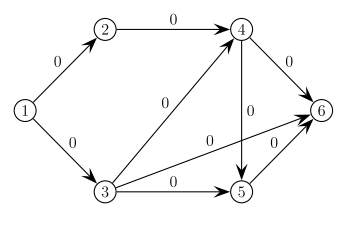
\includegraphics[width=0.5\linewidth,keepaspectratio]{vgraph2}
\end{center}


%$$
%\psset{arrows=->, arrowsize=9pt, labelsep=3pt, mnode=circle}
%\begin{psmatrix}
%&2&&4&[mnode=none] \\
%1&&&&6\\
%&3&&5&[mnode=none]
%\ncline{2,1}{1,2}\naput{0} % 1->2
%\ncline{2,1}{3,2}\naput{0} % 1->3
%\ncline{1,2}{1,4}\naput{0} % 2->4
%\ncline{3,2}{3,4}\naput{0} % 3->5
%\ncline{3,2}{1,4}\naput{0} % 3->4
%\ncline{3,2}{2,5}\naput{0} % 3->6 SINK
%\ncline{1,4}{3,4}\naput{0} % 4->5
%\ncline{1,4}{2,5}\naput{0} % 4->6 SINK
%\ncline{3,4}{2,5}\naput{0} % 5->6 SINK
%\end{psmatrix}
%$$

\end{frame}
%%%%%%%%%%%%%%%%%%%%%%%%%%%%%%%%%%%%%%%%%%%%%%%%%%%%%%%%%%%
\begin{frame}[fragile]{Ford-Fulkerson Algorithm}

Now we need to find an augmenting path.  There are millions of them (well, maybe not exactly millions, I count six).  Let take the path $1\rightarrow 3\rightarrow 6$ to start with.  Now we have to figure out what how much more stuff we can pipe down this route.  The pipe from $1\rightarrow 3$ has capacity $9$ ($c_{1,3}=9$), and is currently piping $0$ ($x_{1,3}=0$ right now), so it could pipe $9$ more.  The pipe from $3\rightarrow 6$ has capacity $2$ and is currently piping $0$, so it could pipe $2$ more.  We can only pipe the minimum of these numbers, so we will only be able to send $2$ units of stuff down this path.

Then we update the flow:

\begin{center}
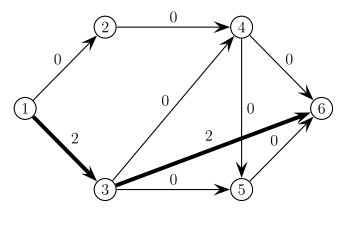
\includegraphics[width=0.5\linewidth,keepaspectratio]{vgraph3}
\end{center}


%$$
%\psset{arrows=->, arrowsize=9pt, labelsep=3pt, mnode=circle}
%\begin{psmatrix}
%&2&&4&[mnode=none] \\
%1&&&&6\\
%&3&&5&[mnode=none]
%\ncline{2,1}{1,2}\naput{0} % 1->2
%\ncline{1,2}{1,4}\naput{0} % 2->4
%\ncline{3,2}{3,4}\naput{0} % 3->5
%\ncline{3,2}{1,4}\naput{0} % 3->4
%\ncline{1,4}{3,4}\naput{0} % 4->5
%\ncline{1,4}{2,5}\naput{0} % 4->6 SINK
%\ncline{3,4}{2,5}\naput{0} % 5->6 SINK
%\psset{linewidth=3pt}
%\ncline{2,1}{3,2}\naput{2} % 1->3
%\ncline{3,2}{2,5}\naput{2} % 3->6 SINK
%\end{psmatrix}
%$$

\end{frame}
%%%%%%%%%%%%%%%%%%%%%%%%%%%%%%%%%%%%%%%%%%%%%%%%%%%%%%%%%%%
\begin{frame}[fragile]{Ford-Fulkerson Algorithm}

We are now ready to repeat.  Let's take the augmenting path $1\rightarrow 3\rightarrow 5\rightarrow 6$.  For each arc we check how much spare capacity it has:
$$
\begin{array}{r|ccccc}
\mbox{arc}&\mbox{total capacity}&&\mbox{current load}&&\mbox{excess capacity}\\
\hline
1\rightarrow 3&9&-&2&=&7\\
3\rightarrow 5&3&-&0&=&3\\
5\rightarrow 6&9&-&0&=&9
\end{array}
$$

\end{frame}
%%%%%%%%%%%%%%%%%%%%%%%%%%%%%%%%%%%%%%%%%%%%%%%%%%%%%%%%%%%
\begin{frame}[fragile]{Ford-Fulkerson Algorithm}

The smallest excess capacity is $3$, so that's what we'll add to the flow, which is shown below:

\begin{center}
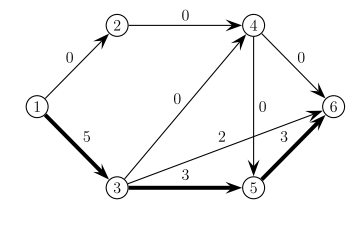
\includegraphics[width=0.5\linewidth,keepaspectratio]{vgraph4}
\end{center}

%$$
%\psset{arrows=->, arrowsize=9pt, labelsep=3pt, mnode=circle}
%\begin{psmatrix}
%&2&&4&[mnode=none] \\
%1&&&&6\\
%&3&&5&[mnode=none]
%\ncline{2,1}{1,2}\naput{0} % 1->2
%\ncline{1,2}{1,4}\naput{0} % 2->4
%\ncline{3,2}{1,4}\naput{0} % 3->4
%\ncline{1,4}{3,4}\naput{0} % 4->5
%\ncline{1,4}{2,5}\naput{0} % 4->6 SINK
%\ncline{3,2}{2,5}\naput{2} % 3->6 SINK
%\psset{linewidth=3pt}
%\ncline{2,1}{3,2}\naput{5} % 1->3
%\ncline{3,2}{3,4}\naput{3} % 3->5
%\ncline{3,4}{2,5}\naput{3} % 5->6 SINK
%\end{psmatrix}
%$$

\end{frame}
%%%%%%%%%%%%%%%%%%%%%%%%%%%%%%%%%%%%%%%%%%%%%%%%%%%%%%%%%%%
\begin{frame}[fragile]{Ford-Fulkerson Algorithm}

Time for another augmenting path.  This time let's take $1\rightarrow 2\rightarrow 4\rightarrow 6$.  The excess capacities of these arcs are $5$, $4$, and $3$, respectively, so the most we can send down this way is $3$.  The updated flow is:

\begin{center}
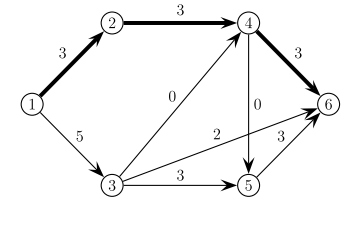
\includegraphics[width=0.5\linewidth,keepaspectratio]{vgraph5}
\end{center}
%$$
%\psset{arrows=->, arrowsize=9pt, labelsep=3pt, mnode=circle}
%\begin{psmatrix}
%&2&&4&[mnode=none] \\
%1&&&&6\\
%&3&&5&[mnode=none]
%\ncline{3,2}{1,4}\naput{0} % 3->4
%\ncline{1,4}{3,4}\naput{0} % 4->5
%\ncline{3,2}{2,5}\naput{2} % 3->6 SINK
%\ncline{2,1}{3,2}\naput{5} % 1->3
%\ncline{3,2}{3,4}\naput{3} % 3->5
%\ncline{3,4}{2,5}\naput{3} % 5->6 SINK
%\psset{linewidth=3pt}
%\ncline{2,1}{1,2}\naput{3} % 1->2
%\ncline{1,2}{1,4}\naput{3} % 2->4
%\ncline{1,4}{2,5}\naput{3} % 4->6 SINK
%\end{psmatrix}
%$$

\end{frame}
%%%%%%%%%%%%%%%%%%%%%%%%%%%%%%%%%%%%%%%%%%%%%%%%%%%%%%%%%%%
\begin{frame}[fragile]{Ford-Fulkerson Algorithm}

It's getting a little harder to spot augmenting paths now, but there's at least one more: $1\rightarrow 2\rightarrow 4\rightarrow 5\rightarrow 6$.  We have
$$
\begin{array}{r|ccccc}
\mbox{arc}&\mbox{total capacity}&&\mbox{current load}&&\mbox{excess capacity}\\
\hline
1\rightarrow 2&5&-&3&=&2\\
2\rightarrow 4&4&-&3&=&1\\
4\rightarrow 5&1&-&0&=&1\\
5\rightarrow 6&9&-&3&=&6
\end{array}
$$
This shows that we can send one unit of stuff down this path.  The updated flow is
\begin{center}
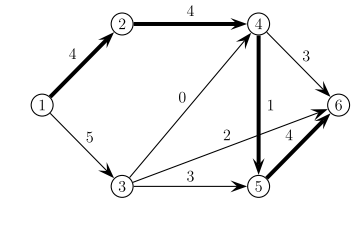
\includegraphics[width=0.5\linewidth,keepaspectratio]{vgraph6}
\end{center}
%$$
%\psset{arrows=->, arrowsize=9pt, labelsep=3pt, mnode=circle}
%\begin{psmatrix}
%&2&&4&[mnode=none] \\
%1&&&&6\\
%&3&&5&[mnode=none]
%\ncline{3,2}{1,4}\naput{0} % 3->4
%\ncline{3,2}{2,5}\naput{2} % 3->6 SINK
%\ncline{2,1}{3,2}\naput{5} % 1->3
%\ncline{3,2}{3,4}\naput{3} % 3->5
%\ncline{1,4}{2,5}\naput{3} % 4->6 SINK
%\psset{linewidth=3pt}
%\ncline{2,1}{1,2}\naput{4} % 1->2
%\ncline{1,2}{1,4}\naput{4} % 2->4
%\ncline{1,4}{3,4}\naput{1} % 4->5
%\ncline{3,4}{2,5}\naput{4} % 5->6 SINK
%\end{psmatrix}
%$$

\end{frame}
%%%%%%%%%%%%%%%%%%%%%%%%%%%%%%%%%%%%%%%%%%%%%%%%%%%%%%%%%%%
\begin{frame}[fragile]{Ford-Fulkerson Algorithm}


Now we're managing to get $9$ units from the source to the sink.  But, is the best we can do?

\bigskip
{\bf How you know when you're done}
\bigskip

Trying to move stuff from the source to the sink depends very much on the paths from the source to the sink.  It is depends on the ways in which those paths can be cut off.

\begin{definition}
A {\it cut\/} in a network (or just a digraph) is a set of arcs such that if they are removed, there is not path from the source to the sink.
\end{definition}

\end{frame}
%%%%%%%%%%%%%%%%%%%%%%%%%%%%%%%%%%%%%%%%%%%%%%%%%%%%%%%%%%%
\begin{frame}[fragile]{Ford-Fulkerson Algorithm}

For example, the dashed arcs in our graph below represent a cut since removing them leaves no paths from the source to the sink.  (Note that you are {\it not\/} allowed to go $1\rightarrow 3\rightarrow5\rightarrow4\rightarrow6$, because then you are traversing the $4\rightarrow 6$ arc in the wrong direction.)

\begin{center}
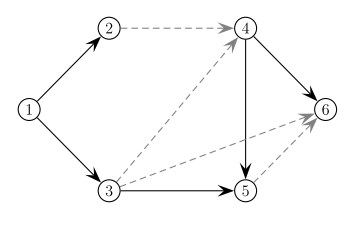
\includegraphics[width=0.5\linewidth,keepaspectratio]{vgraph7}
\end{center}

%$$
%\psset{arrows=->, arrowsize=9pt, labelsep=3pt, mnode=circle}
%\begin{psmatrix}
%&2&&4&[mnode=none] \\
%1&&&&6\\
%&3&&5&[mnode=none]
%\ncline{2,1}{3,2} % 1->3
%\ncline{3,2}{3,4} % 3->5
%\ncline{1,4}{2,5} % 4->6 SINK
%\ncline{2,1}{1,2} % 1->2
%\ncline{1,4}{3,4} % 4->5
%\psset{linecolor=gray, linestyle=dashed}
%\ncline{1,2}{1,4} % 2->4
%\ncline{3,4}{2,5} % 5->6 SINK
%\ncline{3,2}{2,5} % 3->6 SINK
%\ncline{3,2}{1,4} % 3->4
%\end{psmatrix}
%$$

\end{frame}
%%%%%%%%%%%%%%%%%%%%%%%%%%%%%%%%%%%%%%%%%%%%%%%%%%%%%%%%%%%
\begin{frame}[fragile]{Ford-Fulkerson Algorithm}

We will need to measure how much stuff could flow through all the arcs in a cut:

\begin{definition}
The {\it capacity\/} of a cut is defined to be the sum of the capacities of every arc in the cut.
\end{definition}

So to figure out the capacity of a cut, we want to look at the original capacity graph, {\it not\/} the flow graph we may or may not have just made.  The example cut above, shown on the capacity graph below, has capacity $4+8+2+9=23$.

\begin{center}
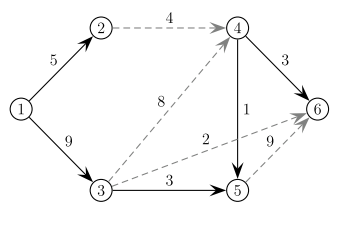
\includegraphics[width=0.5\linewidth,keepaspectratio]{vgraph8}
\end{center}

%$$
%\psset{arrows=->, arrowsize=9pt, labelsep=3pt, mnode=circle}
%\begin{psmatrix}
%&2&&4&[mnode=none] \\
%1&&&&6\\
%&3&&5&[mnode=none]
%\ncline{2,1}{1,2}\naput{5} % 1->2
%\ncline{2,1}{3,2}\naput{9} % 1->3
%\ncline{3,2}{3,4}\naput{3} % 3->5
%\ncline{1,4}{3,4}\naput{1} % 4->5
%\ncline{1,4}{2,5}\naput{3} % 4->6 SINK
%\psset{linecolor=gray, linestyle=dashed}
%\ncline{1,2}{1,4}\naput{4} % 2->4
%\ncline{3,2}{1,4}\naput{8} % 3->4
%\ncline{3,2}{2,5}\naput{2} % 3->6 SINK
%\ncline{3,4}{2,5}\naput{9} % 5->6 SINK
%\end{psmatrix}
%$$

\end{frame}
%%%%%%%%%%%%%%%%%%%%%%%%%%%%%%%%%%%%%%%%%%%%%%%%%%%%%%%%%%%
\begin{frame}[fragile]{Ford-Fulkerson Algorithm}

Now we are ready for the big theorem, which will tell us when we are done in the Ford-Fulkerson Algorithm.

\begin{theorem}[Max-Flow Min-Cut Theorem]
In every network, the maximum flow equals the minimum capacity of a cut.
\end{theorem}

This theorem was proved in 1956 independently by Ford and Fulkerson and by Feinstein and Shannon.  The proof by Ford and Fulkerson uses their algorithm is a very straight-forward way.  The theorem can also be proved by apply the Duality Theorem from Linear Programming.

The only problem with the Max-Flow Min-Cut Theorem is that the two quantities it says are equal are both hard to get a handle on.  But, it is nice to know that if you can find a flow and a cut with the same value, you are done.  That is, you have found the best flow possible for that network.

What about our example?  Did we find the best flow possible?  Well, we were able to pump $9$ units from the source to the sink.  However, the cut we found had capacity $23$, so there must either be a better flow or a smaller cut.  Let's keep playing around with the cuts for a while, and see if we can make a better one.

\end{frame}
%%%%%%%%%%%%%%%%%%%%%%%%%%%%%%%%%%%%%%%%%%%%%%%%%%%%%%%%%%%
\begin{frame}[fragile]{Ford-Fulkerson Algorithm}

Here's a cut with capacity $5+9=14$:

\begin{center}
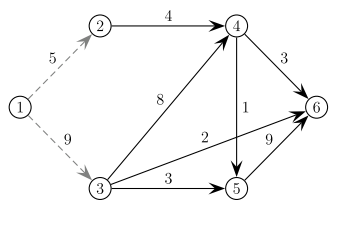
\includegraphics[width=0.5\linewidth,keepaspectratio]{vgraph9}
\end{center}


%$$
%\psset{arrows=->, arrowsize=9pt, labelsep=3pt, mnode=circle}
%\begin{psmatrix}
%&2&&4&[mnode=none] \\
%1&&&&6\\
%&3&&5&[mnode=none]
%\ncline{3,2}{3,4}\naput{3} % 3->5
%\ncline{1,4}{3,4}\naput{1} % 4->5
%\ncline{1,4}{2,5}\naput{3} % 4->6 SINK
%\ncline{1,2}{1,4}\naput{4} % 2->4
%\ncline{3,2}{1,4}\naput{8} % 3->4
%\ncline{3,2}{2,5}\naput{2} % 3->6 SINK
%\ncline{3,4}{2,5}\naput{9} % 5->6 SINK
%\psset{linecolor=gray, linestyle=dashed}
%\ncline{2,1}{1,2}\naput{5} % 1->2
%\ncline{2,1}{3,2}\naput{9} % 1->3
%\end{psmatrix}
%$$

\end{frame}
%%%%%%%%%%%%%%%%%%%%%%%%%%%%%%%%%%%%%%%%%%%%%%%%%%%%%%%%%%%
\begin{frame}[fragile]{Ford-Fulkerson Algorithm}

And here's another cut with capacity $3+2+9=14$:

\begin{center}
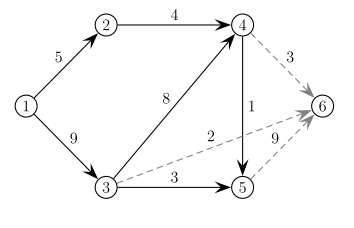
\includegraphics[width=0.5\linewidth,keepaspectratio]{vgraph10}
\end{center}


%$$
%\psset{arrows=->, arrowsize=9pt, labelsep=3pt, mnode=circle}
%\begin{psmatrix}
%&2&&4&[mnode=none] \\
%1&&&&6\\
%&3&&5&[mnode=none]
%\ncline{2,1}{1,2}\naput{5} % 1->2
%\ncline{2,1}{3,2}\naput{9} % 1->3
%\ncline{3,2}{3,4}\naput{3} % 3->5
%\ncline{1,4}{3,4}\naput{1} % 4->5
%\ncline{1,2}{1,4}\naput{4} % 2->4
%\ncline{3,2}{1,4}\naput{8} % 3->4
%\psset{linecolor=gray, linestyle=dashed}
%\ncline{1,4}{2,5}\naput{3} % 4->6 SINK
%\ncline{3,2}{2,5}\naput{2} % 3->6 SINK
%\ncline{3,4}{2,5}\naput{9} % 5->6 SINK
%\end{psmatrix}
%$$

\end{frame}
%%%%%%%%%%%%%%%%%%%%%%%%%%%%%%%%%%%%%%%%%%%%%%%%%%%%%%%%%%%
\begin{frame}[fragile]{Ford-Fulkerson Algorithm}

Finally, here's a tricky cut with capacity $2+1+3+3=9$:

\begin{center}
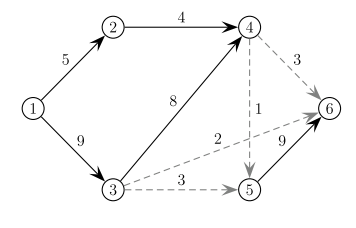
\includegraphics[width=0.5\linewidth,keepaspectratio]{vgraph11}
\end{center}

So, we found a flow that transported $9$ units and a cut that had capacity $9$.  By the Max-Flow Min-Cut Theorem we have found the best flow possible, and we can stop.


%$$
%\psset{arrows=->, arrowsize=9pt, labelsep=3pt, mnode=circle}
%\begin{psmatrix}
%&2&&4&[mnode=none] \\
%1&&&&6\\
%&3&&5&[mnode=none]
%\ncline{2,1}{1,2}\naput{5} % 1->2
%\ncline{2,1}{3,2}\naput{9} % 1->3
%\ncline{1,2}{1,4}\naput{4} % 2->4
%\ncline{3,2}{1,4}\naput{8} % 3->4
%\ncline{3,4}{2,5}\naput{9} % 5->6 SINK
%\psset{linecolor=gray, linestyle=dashed}
%\ncline{1,4}{2,5}\naput{3} % 4->6 SINK
%\ncline{1,4}{3,4}\naput{1} % 4->5
%\ncline{3,2}{2,5}\naput{2} % 3->6 SINK
%\ncline{3,2}{3,4}\naput{3} % 3->5
%\end{psmatrix}
%$$

\end{frame}
%%%%%%%%%%%%%%%%%%%%%%%%%%%%%%%%%%%%%%%%%%%%%%%%%%%%%%%%%%%
\begin{frame}[fragile]{Wrinkles}


Let's suppose now that the capacity graph is

\begin{center}
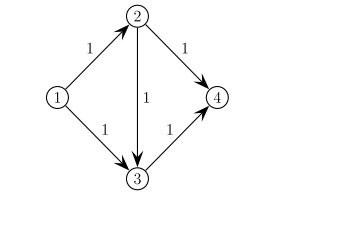
\includegraphics[width=0.5\linewidth,keepaspectratio]{vgraph12}
\end{center}



%$$
%\psset{arrows=->, arrowsize=9pt, labelsep=3pt, mnode=circle}
%\begin{psmatrix}
%&2&[mnode=none] \\
%1&&4\\
%&3&[mnode=none]
%\ncline{2,1}{1,2}\naput{1} % 1->2
%\ncline{2,1}{3,2}\naput{1} % 1->3
%\ncline{1,2}{2,3}\naput{1} % 2->4
%\ncline{3,2}{2,3}\naput{1} % 3->4
%\ncline{1,2}{3,2}\naput{1} % 2->3
%\end{psmatrix}
%$$

\end{frame}
%%%%%%%%%%%%%%%%%%%%%%%%%%%%%%%%%%%%%%%%%%%%%%%%%%%%%%%%%%%
\begin{frame}[fragile]{Wrinkles}

And let's suppose that we start the Ford-Fulkerson Algorithm by adding the augmenting path $1\rightarrow2\rightarrow3\rightarrow4$, which we can ship $1$ unit down.  Then we get the following flow


\begin{center}
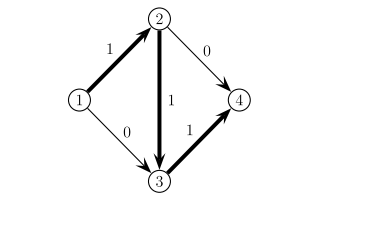
\includegraphics[width=0.5\linewidth,keepaspectratio]{vgraph13}
\end{center}


%$$
%\psset{arrows=->, arrowsize=9pt, labelsep=3pt, mnode=circle}
%\begin{psmatrix}
%&2&[mnode=none] \\
%1&&4\\
%&3&[mnode=none]
%\ncline{2,1}{3,2}\naput{0} % 1->3
%\ncline{1,2}{2,3}\naput{0} % 2->4
%\psset{linewidth=3pt}
%\ncline{2,1}{1,2}\naput{1} % 1->2
%\ncline{3,2}{2,3}\naput{1} % 3->4
%\ncline{1,2}{3,2}\naput{1} % 2->3
%\end{psmatrix}
%$$

\end{frame}
%%%%%%%%%%%%%%%%%%%%%%%%%%%%%%%%%%%%%%%%%%%%%%%%%%%%%%%%%%%
\begin{frame}[fragile]{Wrinkles}

Stop for a moment and answer these questions: Is this the maximum flow possible?  If not, can you spot an augmenting path that would make it maximum?

To answer the first question you should think of the Max-Flow Min-Cut Theorem.  If we could find a cut of capacity $1$, then this would indeed be the maximum possible flow.  Sadly, there is no cut of capacity $1$.  Then minimum cut we can make has capacity $2$:

\begin{center}
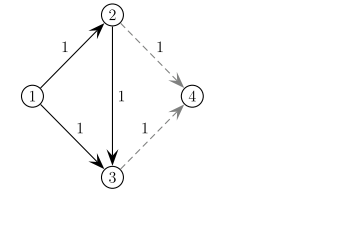
\includegraphics[width=0.5\linewidth,keepaspectratio]{vgraph14}
\end{center}


%$$
%\psset{arrows=->, arrowsize=9pt, labelsep=3pt, mnode=circle}
%\begin{psmatrix}
%&2&[mnode=none] \\
%1&&4\\
%&3&[mnode=none]
%\ncline{2,1}{1,2}\naput{1} % 1->2
%\ncline{2,1}{3,2}\naput{1} % 1->3
%\ncline{1,2}{3,2}\naput{1} % 2->3
%\psset{linecolor=gray, linestyle=dashed}
%\ncline{1,2}{2,3}\naput{1} % 2->4
%\ncline{3,2}{2,3}\naput{1} % 3->4
%\end{psmatrix}
%$$

\end{frame}
%%%%%%%%%%%%%%%%%%%%%%%%%%%%%%%%%%%%%%%%%%%%%%%%%%%%%%%%%%%
\begin{frame}[fragile]{Wrinkles}

The Max-Flow Min-Cut Theorem then tells us that there must be a better flow.  Of course, in this example, it's easy to find a better flow, but don't think about that.  The concern right now is: how can we improve the flow we already have?

The answer is that we can add an augmenting path that goes the wrong way down a pipe!  So, we can add the path that goes $1\rightarrow 3\rightarrow 2\rightarrow 4$.  But how much can we take through this route?

We compute excess capacity like normal for the arcs that we are going the right way on:
$$
\begin{array}{r|ccccc}
\mbox{arc}&\mbox{total capacity}&&\mbox{current load}&&\mbox{excess capacity}\\
\hline
1\rightarrow 3&1&-&0&=&1\\
2\rightarrow 4&1&-&0&=&1
\end{array}
$$

\end{frame}
%%%%%%%%%%%%%%%%%%%%%%%%%%%%%%%%%%%%%%%%%%%%%%%%%%%%%%%%%%%
\begin{frame}[fragile]{Wrinkles}

For the $3\rightarrow 2$ arc that we are going the wrong way down, the excess capacity is however much is currently flowing down it in the right direction.  So, since we are currently sending $1$ unit down the $2\rightarrow 3$ arc in the right direction (that is, from $2$ to $3$), we can send $1$ unit up this arc in the wrong direction.

Then the other change is that when we update the flow, we add the new amount to the arcs that we went down in the right direction like before, but we {\it subtract\/} the new amount from the arcs that we went down the wrong way.

In this case our new flow is

\begin{center}
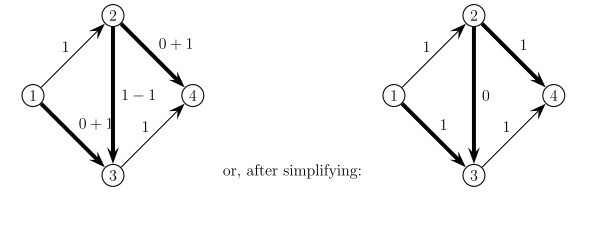
\includegraphics[width=0.9\linewidth,keepaspectratio]{vgraph15}
\end{center}


%$$
%\begin{array}{ccc}
%
%\psset{arrows=->, arrowsize=9pt, labelsep=3pt, mnode=circle}
%\begin{psmatrix}
%&2&[mnode=none] \\
%1&&4\\
%&3&[mnode=none]
%\ncline{2,1}{1,2}\naput{1} % 1->2
%\ncline{3,2}{2,3}\naput{1} % 3->4
%\psset{linewidth=3pt}
%\ncline{2,1}{3,2}\naput{0+1} % 1->3
%\ncline{1,2}{2,3}\naput{0+1} % 2->4
%\ncline{1,2}{3,2}\naput{1-1} % 2->3
%\end{psmatrix}
%
%
%&\mbox{ or, after simplifying: }&
%
%\psset{arrows=->, arrowsize=9pt, labelsep=3pt, mnode=circle}
%\begin{psmatrix}
%&2&[mnode=none] \\
%1&&4\\
%&3&[mnode=none]
%\ncline{2,1}{1,2}\naput{1} % 1->2
%\ncline{3,2}{2,3}\naput{1} % 3->4
%\psset{linewidth=3pt}
%\ncline{2,1}{3,2}\naput{1} % 1->3
%\ncline{1,2}{2,3}\naput{1} % 2->4
%\ncline{1,2}{3,2}\naput{0} % 2->3
%\end{psmatrix}
%\end{array}
%$$

\end{frame}
%%%%%%%%%%%%%%%%%%%%%%%%%%%%%%%%%%%%%%%%%%%%%%%%%%%%%%%%%%%
\begin{frame}[fragile]{Wrinkles}

This has now increased our total flow to $2$, and since we already found a cut of capacity $2$, the Max-Flow Min-Cut Theorem tells us that we are done.

There are two ways to think about why we are allowed to send stuff the wrong way down a pipe.  First, we might just observe that in adding the augmenting path in the manner in which we just did, we did break any of the rules for flows - that is, our new flow still satisfied (\ref{flow1}), (\ref{flow2}), and (\ref{flow3}).

The other way to think about it is that instead of ``sending stuff the wrong way,'' we were really just dropping off stuff on one side of the arc and then telling the previous path to leave it's stuff on the other side of the arc.  In our example, in our initial flow we were pumping $1$ unit from $1$ to $2$ to $3$ to $4$.  When we went to add the new path, what we said to the old path was ``we'll bring one unit from $1$ to $3$, so you can take that to $4$, and hey, would you mind leaving a unit at $2$ so that we can pick it up and take it to $4$?''

\end{frame}



%   \begin{frame}[fragile]
%\frametitle{Adjacency matrix}
%
%
%\end{frame}
%
%   \begin{frame}[fragile]
%\frametitle{Dijkstra's Algorithm on adjacency matrix}
%
% \begin{center}
% \begin{tabular}{|l|c|c|c|c|c|c|}
% \hline
% & Charlotte &  {yellow} Atlanta &   {yellow}Nashville &   {yellow}Knoxville& \textbf{Columbia} &  {yellow}Raleigh\\
% &[52]&  {yellow}[19]&  {yellow}[25]&  {yellow}[37]&[40]& {yellow}[0]\\
% \hline
% Charlotte & * &  {yellow}&  {yellow}&  {yellow}15&14& {yellow}\\
% \hline
%  {yellow} Atlanta &  {yellow}&  {yellow}*&  {yellow}&  {yellow}18&  {yellow}24& {yellow}19\\
% \hline
%  {yellow}Nashville&  {yellow}&  {yellow}&  {yellow}*&  {yellow}18&  {yellow}15& {yellow}25\\
% \hline
%   {yellow}Knoxville &  {yellow}15&  {yellow}18&  {yellow}18&  {yellow}*&  {yellow}14& {yellow}\\
% \hline
% Columbia & 14 &   {yellow}24&  {yellow}15&  {yellow}14&8& {yellow}\\
% \hline
%  {yellow}Raleigh & {yellow}& {yellow}19& {yellow}25& {yellow}& {yellow}& {yellow}*\\
% \hline
% \end{tabular}
% \end{center}
% 
%\end{frame}

%%%%Euler circuits
%\begin{definition}[Loop]
%A \textbf{loop} is a special type of edge that connects a vertex to itself.  %Loops are not used much in street network graphs.
%\end{definition}
%
%   \begin{frame}[fragile]
%\frametitle{Euler path and circuit}
%\begin{definition}[Euler Path]
%\begin{enumerate}
%\item 
%An \textbf{Euler path} is a path that uses every edge in a graph with no repeats.  Being a path, it does not have to return to the starting vertex.
%\item An \textbf{Euler circuit} is a circuit that uses every edge in a graph with no repeats.  Being a circuit, it must start and end at the same vertex.
%\end{enumerate}
%\end{definition}
% 
%\begin{theorem}[Euler's Path and Circuit Theorems]
%\begin{itemize}
%\item A graph will contain an Euler path if it contains at most two vertices of odd degree.
%\item A graph will contain an Euler circuit if all vertices have even degree
%\end{itemize}
%\end{theorem}
%\end{frame}
%
%%%%%Eulerization and Chinese Postman Problem
%   \begin{frame}[fragile]
%\frametitle{Euler example}
%\begin{center}
%\begin{tikzpicture}
%\draw[blue] (0,0)--(0,-2);
%\draw[fill] (0,-2) circle[radius=.1];
%\draw[blue] (0,0) -- (0,2);
%\draw[fill] (0,0) circle[radius=.1];
%\draw[fill] (0,2) circle[radius=.1];
%\draw[blue] (0,0)--(3,0);
%\draw[fill] (3,0) circle[radius=.1];
%\draw[blue] (3,0)--(6,0);
%\draw[fill] (6,0) circle[radius=.1];
%\draw[fill] (6,2) circle[radius=.1];
%\draw[blue] (6,2)--(6,0);
%\draw[blue] (3,2)--(3,0);
%\draw[blue] (6,-2)--(6,0);
%\draw[fill] (6,-2) circle[radius=.1];
%\draw[fill] (3,2) circle[radius=.1];
%\draw[blue] (6,-2)--(6,0);
%\draw[blue] (6,-2)--(3,0);
%\draw[blue] (0,-2)--(3,0);
%\draw[blue] (3,2)--(6,2);
%\draw[blue] (0,2)--(3,0);
%\draw[blue] (6,0)--(3,2);
%\draw[blue] (3,2)--(0,0);
%%\draw[red] (2,-2)--(3,0);
%\end{tikzpicture}
%\end{center}
%\end{frame}
%
%
%   \begin{frame}[fragile]
%\frametitle{Euler example}
%\begin{center}
%\begin{tikzpicture}
%\draw[blue] (0,0)--(0,-2);
%\draw[fill] (0,-2) circle[radius=.1] node[left]{2};
%\draw[blue] (0,0) -- (0,2);
%\draw[fill] (0,0) circle[radius=.1] node[left]{4};
%\draw[fill] (0,2) circle[radius=.1] node[left]{2};
%\draw[blue] (0,0)--(3,0);
%\draw[fill] (3,0) circle[radius=.1] node[below]{6};
%\draw[blue] (3,0)--(6,0);
%\draw[fill] (6,0) circle[radius=.1] node[right]{4};
%\draw[fill] (6,2) circle[radius=.1] node[right]{2};
%\draw[blue] (6,2)--(6,0);
%\draw[blue] (3,2)--(3,0);
%\draw[blue] (6,-2)--(6,0);
%\draw[fill] (6,-2) circle[radius=.1] node[right]{2};
%\draw[fill] (3,2) circle[radius=.1] node[above]{4};
%\draw[blue] (6,-2)--(6,0);
%\draw[blue] (6,-2)--(3,0);
%\draw[blue] (0,-2)--(3,0);
%\draw[blue] (3,2)--(6,2);
%\draw[blue] (0,2)--(3,0);
%\draw[blue] (6,0)--(3,2);
%\draw[blue] (3,2)--(0,0);
%%\draw[red] (2,-2)--(3,0);
%\end{tikzpicture}
%\end{center}
%\end{frame}
%
%
%   \begin{frame}[fragile]
%\frametitle{Eulerization}
%\begin{definition}[Eulerization]
%\textbf{Eulerization} is the process of adding edges to a graph to create an Euler circuit on a graph.  To eulerize a graph, edges are duplicated to connect pairs of vertices with odd degree.  Connecting two odd degree vertices increases the degree of each, giving them both even degree.  When two odd degree vertices are not directly connected, we can duplicate all edges in a path connecting the two.
%\end{definition}
%\end{frame}
%
%   \begin{frame}[fragile]
%\frametitle{Chinese Postman Problem}
%\begin{center}
%\begin{tikzpicture}
%
%\draw[blue] (0,0)--(2,-2);
%\draw[fill] (2,-2) circle[radius=.1];
%\draw[blue] (0,0) -- (1,1);
%\draw[fill] (0,0) circle[radius=.1];
%\draw[fill] (1,1) circle[radius=.1];
%\draw[blue] (0,0)--(3,0);
%\draw[fill] (3,0) circle[radius=.1];
%\draw[blue] (3,0)--(6,0);
%\draw[fill] (6,0) circle[radius=.1];
%\draw[fill] (5,2) circle[radius=.1];
%\draw[blue] (5,2)--(1,1);
%\draw[blue] (5,2)--(6,0);
%\draw[blue] (5,2)--(3,0);
%\draw[fill] (6,-2) circle[radius=.1];
%\draw[fill] (5,-1) circle[radius=.1];
%\draw[blue] (6,-2)--(6,0);
%\draw[blue] (5,-1)--(6,0);
%\draw[blue] (6,-2)--(2,-2);
%\draw[blue] (5,-1)--(2,-2);
%%\draw[red] (2,-2)--(3,0);
%\end{tikzpicture}
%\end{center}
%
%
%
%\end{frame}
%
%   \begin{frame}[fragile]
%\frametitle{Chinese Postman Problem}
%
%\begin{center}
%\begin{tikzpicture}
%
%\draw[blue] (0,0)--(2,-2);
%\draw[fill] (2,-2) circle[radius=.1] node [left]{3};
%\draw[blue] (0,0) -- (1,1);
%\draw[fill] (0,0) circle[radius=.1] node [left]{3};
%\draw[fill] (1,1) circle[radius=.1] node [left]{2};
%\draw[blue] (0,0)--(3,0);
%\draw[fill] (3,0) circle[radius=.1] node [above]{3};
%\draw[blue] (3,0)--(6,0);
%\draw[fill] (6,0) circle[radius=.1] node [right]{4};
%\draw[fill] (5,2) circle[radius=.1] node [right]{3};
%\draw[blue] (5,2)--(1,1);
%\draw[blue] (5,2)--(6,0);
%\draw[blue] (5,2)--(3,0);
%\draw[fill] (6,-2) circle[radius=.1] node [right]{2};
%\draw[fill] (5,-1) circle[radius=.1] node [below]{2};
%\draw[blue] (6,-2)--(6,0);
%\draw[blue] (5,-1)--(6,0);
%\draw[blue] (6,-2)--(2,-2);
%\draw[blue] (5,-1)--(2,-2);
%%\draw[red] (2,-2)--(3,0);
%\end{tikzpicture}
%\end{center}
%
%\end{frame}
%
%   \begin{frame}[fragile]
%\frametitle{Chinese Postman Problem}
%
%\begin{center}
%\begin{tikzpicture}
%
%\draw[blue] (6,-2)--(6,0);
%\draw[blue] (5,-1)--(6,0);
%\draw[blue] (6,-2)--(2,-2);
%\draw[blue] (5,-1)--(2,-2);
%\draw[blue] (5,2)--(1,1);
%\draw[blue] (5,2)--(6,0);
%\draw[blue] (5,2)--(3,0);
%\draw[blue] (3,0)--(6,0);
%\draw[blue] (0,0)--(3,0);
%\draw[blue] (0,0) -- (1,1);
%\draw[red] (0,0) to [out=-45, in=-45] (3,0);
%\draw[blue] (0,0)--(2,-2);
%\draw[fill] (2,-2) circle[radius=.1] node [left]{3};
%\draw[fill] (0,0) circle[radius=.1] node [left]{4};
%\draw[fill] (1,1) circle[radius=.1] node [left]{2};
%\draw[fill] (3,0) circle[radius=.1] node [above]{4};
%\draw[fill] (6,0) circle[radius=.1] node [right]{4};
%\draw[fill] (5,2) circle[radius=.1] node [right]{3};
%\draw[fill] (6,-2) circle[radius=.1] node [right]{2};
%\draw[fill] (5,-1) circle[radius=.1] node [below]{2};
%
%\end{tikzpicture}
%\end{center}
%
%\end{frame}
%
%%%%%%Hamilton paths and Traveling Salesman (Brute force and nearest neighbor and RNNA and sorted edges algorithm)
%   \begin{frame}[fragile]
%\frametitle{Hamilton paths and circuits}
%\begin{definition}[Complete Graph]
%A \textbf{complete graph} on $n$ vertices contains exactly one edge between every pair of vertices.
%\end{definition}
% 
%
%\begin{definition}[Hamiltonian Circuits and Paths]
%A Hamiltonian circuit is a circuit that visits every vertex once with no repeats.  A Hamiltonian path also visits every vertex once with no repeats, but does not have to start and end at the same vertex.  
%\end{definition}
%
%
%\begin{center}
%\scalebox{.7}{
%\begin{tikzpicture}
%\draw[fill] (0,0) circle[radius=.1] node [left]{B};
%\draw[fill] (4,0) circle[radius=.1] node [right]{C};
%\draw[fill] (2,2) circle[radius=.1] node [right]{D};
%\draw[fill] (2,4) circle[radius=.1] node [above]{A};
%\draw(0,0)--(4,0);
%\draw(0,0)--(2,2);
%\draw(0,0)--(2,4);
%\draw(4,0)--(2,2);
%\draw(4,0)--(2,4);
%\draw(2,4)--(2,2);
%\node at (2,-0.3){13};
%\node at (0.7,1){9};
%\node at (0.7,2){4};
%\node at (3.3,1){8};
%\node at (3.3,2){2};
%\node at (2.2,2.9){1};
%
%\end{tikzpicture}
%}
%\end{center}
%\end{frame}
%
%   \begin{frame}[fragile]
%\frametitle{Nearest Neighbor Algorithm (NNA)}
%\begin{enumerate}
%\item	Select a starting point.
%\item	Move to the nearest unvisited vertex (the edge with smallest weight).
%\item	Repeat until the circuit is complete.
%\end{enumerate}
% 
%\begin{center}
%\scalebox{.7}{
%\begin{tikzpicture}
%\draw[fill] (0,0) circle[radius=.1] node [left]{B};
%\draw[fill] (4,0) circle[radius=.1] node [right]{C};
%\draw[fill] (2,2) circle[radius=.1] node [right]{D};
%\draw[fill] (2,4) circle[radius=.1] node [above]{A};
%\draw(0,0)--(4,0);
%\draw(0,0)--(2,2);
%\draw(0,0)--(2,4);
%\draw(4,0)--(2,2);
%\draw(4,0)--(2,4);
%\draw(2,4)--(2,2);
%\node at (2,-0.3){13};
%\node at (0.7,1){9};
%\node at (0.7,2){4};
%\node at (3.3,1){8};
%\node at (3.3,2){2};
%\node at (2.2,2.9){1};
%\end{tikzpicture}
%}
%\end{center}
%
%\end{frame}
%
%
%   \begin{frame}[fragile]
%\frametitle{Nearest Neighbor Algorithm (NNA)}
%\begin{enumerate}
%\item	Select a starting point.
%\item	Move to the nearest unvisited vertex (the edge with smallest weight).
%\item	Repeat until the circuit is complete.
%\end{enumerate}
% 
%\begin{center}
%\scalebox{.7}{
%\begin{tikzpicture}
%\draw[fill] (0,0) circle[radius=.1] node [left]{B};
%\draw[fill] (4,0) circle[radius=.1] node [right]{C};
%\draw[fill] (2,2) circle[radius=.1] node [right]{D};
%\draw[fill] (2,4) circle[radius=.1] node [above]{A};
%\draw[very thick, blue] (0,0)--(4,0);
%\draw(0,0)--(2,2);
%\draw[very thick, blue] (0,0)--(2,4);
%\draw[very thick, blue] (4,0)--(2,2);
%\draw(4,0)--(2,4);
%\draw[very thick, blue] (2,4)--(2,2);
%\node at (2,-0.3){13};
%\node at (0.7,1){9};
%\node at (0.7,2){4};
%\node at (3.3,1){8};
%\node at (3.3,2){2};
%\node at (2.2,2.9){1};
%\end{tikzpicture}
%}
%
%
%\textcolor{blue}{$A\rightarrow D \rightarrow C \rightarrow B \rightarrow A$, 26}
%\end{center}
%\end{frame}
%%
%%   \begin{frame}[fragile]
%%\frametitle{NNA Example}
%%picture
%% 
%%It didn't work
%%\end{frame}
%
%   \begin{frame}[fragile]
%\frametitle{Repeated Nearest Neighbor Algorithm (RNNA)}
%\begin{enumerate}
%\item	Do the Nearest Neighbor Algorithm starting at each vertex.
%\item	Choose the circuit produced with minimal total weight.
%\end{enumerate}
% 
%\begin{center}
%$B\rightarrow A \rightarrow D \rightarrow C \rightarrow B$, 26\\
%$C\rightarrow A \rightarrow D \rightarrow B \rightarrow C$, 25\\
%$D\rightarrow A \rightarrow C \rightarrow B \rightarrow D$, 25
%\end{center}
%\end{frame}
%
%
%   \begin{frame}[fragile]
%\frametitle{Repeated Nearest Neighbor Algorithm (RNNA)}
%\begin{enumerate}
%\item	Do the Nearest Neighbor Algorithm starting at each vertex.
%\item	Choose the circuit produced with minimal total weight.
%\end{enumerate}
%\begin{center}
%$B\rightarrow A \rightarrow D \rightarrow C \rightarrow B$, 26\\
%\textcolor{red}{$C\rightarrow A \rightarrow D \rightarrow B \rightarrow C$, 25}\\
%\textcolor{red}{$D\rightarrow A \rightarrow C \rightarrow B \rightarrow D$, 25}
%\end{center}
%\end{frame}
%
%   \begin{frame}[fragile]
%\frametitle{Sorted Edges Algorithm}
%\begin{enumerate}
%\item Select the cheapest unused edge in the graph.
%\item Repeat step 1, adding the cheapest unused edge to the circuit, unless:
%\begin{enumerate}
%\item adding the edge would create a circuit that doesn't contain all vertices, or
%\item adding the edge would give a vertex degree 3.
%\end{enumerate}
%\item Repeat until a circuit containing all vertices is found.
%\end{enumerate}
% 
%\begin{center}
%\scalebox{.7}{
%\begin{tikzpicture}
%\draw[fill] (0,0) circle[radius=.1] node [left]{B};
%\draw[fill] (4,0) circle[radius=.1] node [right]{C};
%\draw[fill] (2,2) circle[radius=.1] node [right]{D};
%\draw[fill] (2,4) circle[radius=.1] node [above]{A};
%\draw(0,0)--(4,0);
%\draw(0,0)--(2,2);
%\draw(0,0)--(2,4);
%\draw(4,0)--(2,2);
%\draw(4,0)--(2,4);
%\draw(2,4)--(2,2);
%\node at (2,-0.3){13};
%\node at (0.7,1){9};
%\node at (0.7,2){4};
%\node at (3.3,1){8};
%\node at (3.3,2){2};
%\node at (2.2,2.9){1};
%\end{tikzpicture}
%}
%\end{center}
%\end{frame}
%%%%%%%%Spanning Trees and min cost
%
%   \begin{frame}[fragile]
%\frametitle{Spanning Tree}
%\begin{definition}[Spanning Tree]
%A spanning tree is a connected graph using all vertices in which there are no circuits.  
%In other words, there is a path from any vertex to any other vertex, but no circuits.   
%\end{definition}
%
% 
%\scalebox{.9}{
%\begin{minipage}{0.2\textwidth}
%\begin{tikzpicture}
%\draw[fill] (0,0) circle[radius=.1];
%\draw[fill] (1,1) circle[radius=.1];
%\draw[fill] (1,2) circle[radius=.1];
%\draw[fill] (2,0) circle[radius=.1];
%\draw(0,0)--(1,2);
%\draw(0,0)--(1,1);
%\draw(1,2)--(2,0);
%\end{tikzpicture}
%\end{minipage}
%%
%\begin{minipage}{0.2\textwidth}
%\begin{tikzpicture}
%\draw[fill] (0,0) circle[radius=.1];
%\draw[fill] (1,1) circle[radius=.1];
%\draw[fill] (1,2) circle[radius=.1];
%\draw[fill] (2,0) circle[radius=.1];
%\draw(0,0)--(1,2);
%\draw(2,0)--(1,1);
%\draw(1,2)--(2,0);
%\end{tikzpicture}
%\end{minipage}
%%
%\begin{minipage}{0.2\textwidth}
%\begin{tikzpicture}
%\draw[fill] (0,0) circle[radius=.1];
%\draw[fill] (1,1) circle[radius=.1];
%\draw[fill] (1,2) circle[radius=.1];
%\draw[fill] (2,0) circle[radius=.1];
%\draw(0,0)--(1,2);
%\draw(0,0)--(1,1);
%\draw(0,0)--(2,0);
%\end{tikzpicture}
%\end{minipage}
%%
%\begin{minipage}{0.2\textwidth}
%\begin{tikzpicture}
%\draw[fill] (0,0) circle[radius=.1];
%\draw[fill] (1,1) circle[radius=.1];
%\draw[fill] (1,2) circle[radius=.1];
%\draw[fill] (2,0) circle[radius=.1];
%\draw(0,0)--(1,2);
%\draw(1,2)--(1,1);
%\draw(1,2)--(2,0);
%\end{tikzpicture}
%\end{minipage}
%%
%\begin{minipage}{0.2\textwidth}
%\begin{tikzpicture}
%\draw[fill] (0,0) circle[radius=.1];
%\draw[fill] (1,1) circle[radius=.1];
%\draw[fill] (1,2) circle[radius=.1];
%\draw[fill] (2,0) circle[radius=.1];
%\draw(1,1)--(1,2);
%\draw(1,2)--(2,0);
%\draw(0,0)--(2,0);
%\end{tikzpicture}
%\end{minipage}}
%
%\end{frame}
%
%
%   \begin{frame}[fragile]
%\frametitle{Kruskal's Algorithm}
%\begin{definition}[Minimum Cost Spanning Tree (MCST)]
%The minimum cost spanning tree is the spanning tree with the smallest total edge weight.  
%\end{definition}
% 
%
%\begin{theorem}[Kruskal's Algorithm]
%\hspace{3in}
%\begin{enumerate}
%\item Select the cheapest unused edge in the graph.
%\item Repeat step 1, adding the cheapest unused edge, unless:
%\begin{enumerate}
%\item adding the edge would create a circuit.
%\end{enumerate}
%\item Repeat until a spanning tree is formed.
%\end{enumerate}
%\end{theorem}
%\end{frame}
%
%   \begin{frame}[fragile]%0
%\frametitle{Example}
%\begin{center}
%\begin{tikzpicture}
%\draw[fill] (0,0) circle[radius=.1] node[below]{D};
%\draw[fill] (3,0) circle[radius=.1] node[below]{C};
%\draw[fill] (-1,1.5) circle[radius=.1] node[left]{E};
%\draw[fill] (2,3) circle[radius=.1] node[above]{A};
%\draw[fill] (5,1.5) circle[radius=.1] node[right]{B};
%\draw(0,0)--(3,0);
%\draw(0,0)--(2,3);
%\draw(0,0)--(-1,1.5);
%\draw(0,0)--(5,1.5);
%\draw(3,0)--(-1,1.5);
%\draw(3,0)--(2,3);
%\draw(3,0)--(5,1.5);
%\draw(-1,1.5)--(2,3);
%\draw(-1,1.5)--(5,1.5);
%\draw(2,3)--(5,1.5);
%\node at (1.5, -0.2){\$7};
%\node at (-0.9, 0.7){\$13};
%\node at (4.6,0.7){\$10};
%\node at (3.5, 2.5){\$4};
%\node at (0.5,2.5){\$5};
%\node at (1.7,1.3){\$6};
%\node at (1.15,2.15){\$9};
%\node at (2.5,2.15){\$8};
%\node at (0,0.9){\$11};
%\node at (3.4,0.85){\$14};
%\end{tikzpicture}
%\end{center}
%\end{frame}
%
%
%   \begin{frame}[fragile]%1
%\frametitle{Example}
%\begin{center}
%\begin{tikzpicture}
%\draw[fill] (0,0) circle[radius=.1] node[below]{D};
%\draw[fill] (3,0) circle[radius=.1] node[below]{C};
%\draw[fill] (-1,1.5) circle[radius=.1] node[left]{E};
%\draw[fill] (2,3) circle[radius=.1] node[above]{A};
%\draw[fill] (5,1.5) circle[radius=.1] node[right]{B};
%\draw(0,0)--(3,0);
%\draw(0,0)--(2,3);
%\draw(0,0)--(-1,1.5);
%\draw(0,0)--(5,1.5);
%\draw(3,0)--(-1,1.5);
%\draw(3,0)--(2,3);
%\draw(3,0)--(5,1.5);
%\draw(-1,1.5)--(2,3);
%\draw(-1,1.5)--(5,1.5);
%\draw[very thick, red](2,3)--(5,1.5);
%\node at (1.5, -0.2){\$7};
%\node at (-0.9, 0.7){\$13};
%\node at (4.6,0.7){\$10};
%\node at (3.5, 2.5){\$4};
%\node at (0.5,2.5){\$5};
%\node at (1.7,1.3){\$6};
%\node at (1.15,2.15){\$9};
%\node at (2.5,2.15){\$8};
%\node at (0,0.9){\$11};
%\node at (3.4,0.85){\$14};
%\end{tikzpicture}
%\end{center}
%\end{frame}
%
%
%   \begin{frame}[fragile]%2
%\frametitle{Example}
%\begin{center}
%\begin{tikzpicture}
%\draw[fill] (0,0) circle[radius=.1] node[below]{D};
%\draw[fill] (3,0) circle[radius=.1] node[below]{C};
%\draw[fill] (-1,1.5) circle[radius=.1] node[left]{E};
%\draw[fill] (2,3) circle[radius=.1] node[above]{A};
%\draw[fill] (5,1.5) circle[radius=.1] node[right]{B};
%\draw(0,0)--(3,0);
%\draw(0,0)--(2,3);
%\draw(0,0)--(-1,1.5);
%\draw(0,0)--(5,1.5);
%\draw(3,0)--(-1,1.5);
%\draw(3,0)--(2,3);
%\draw(3,0)--(5,1.5);
%\draw[very thick, red](-1,1.5)--(2,3);
%\draw(-1,1.5)--(5,1.5);
%\draw[very thick, red](2,3)--(5,1.5);
%\node at (1.5, -0.2){\$7};
%\node at (-0.9, 0.7){\$13};
%\node at (4.6,0.7){\$10};
%\node at (3.5, 2.5){\$4};
%\node at (0.5,2.5){\$5};
%\node at (1.7,1.3){\$6};
%\node at (1.15,2.15){\$9};
%\node at (2.5,2.15){\$8};
%\node at (0,0.9){\$11};
%\node at (3.4,0.85){\$14};
%\end{tikzpicture}
%\end{center}
%\end{frame}
%
%   \begin{frame}[fragile]%3
%\frametitle{Example}
%\begin{center}
%\begin{tikzpicture}
%\draw[fill] (0,0) circle[radius=.1] node[below]{D};
%\draw[fill] (3,0) circle[radius=.1] node[below]{C};
%\draw[fill] (-1,1.5) circle[radius=.1] node[left]{E};
%\draw[fill] (2,3) circle[radius=.1] node[above]{A};
%\draw[fill] (5,1.5) circle[radius=.1] node[right]{B};
%\draw[very thick, red](0,0)--(3,0);
%\draw(0,0)--(2,3);
%\draw(0,0)--(-1,1.5);
%\draw(0,0)--(5,1.5);
%\draw(3,0)--(-1,1.5);
%\draw(3,0)--(2,3);
%\draw(3,0)--(5,1.5);
%\draw[very thick, red](-1,1.5)--(2,3);
%\draw(-1,1.5)--(5,1.5);
%\draw[very thick, red](2,3)--(5,1.5);
%\node at (1.5, -0.2){\$7};
%\node at (-0.9, 0.7){\$13};
%\node at (4.6,0.7){\$10};
%\node at (3.5, 2.5){\$4};
%\node at (0.5,2.5){\$5};
%\node at (1.7,1.3){\$6};
%\node at (1.15,2.15){\$9};
%\node at (2.5,2.15){\$8};
%\node at (0,0.9){\$11};
%\node at (3.4,0.85){\$14};
%\end{tikzpicture}
%\end{center}
%\end{frame}
%
%   \begin{frame}[fragile]%4
%\frametitle{Example}
%\begin{center}
%\begin{tikzpicture}
%\draw[fill] (0,0) circle[radius=.1] node[below]{D};
%\draw[fill] (3,0) circle[radius=.1] node[below]{C};
%\draw[fill] (-1,1.5) circle[radius=.1] node[left]{E};
%\draw[fill] (2,3) circle[radius=.1] node[above]{A};
%\draw[fill] (5,1.5) circle[radius=.1] node[right]{B};
%\draw[very thick, red](0,0)--(3,0);
%\draw(0,0)--(2,3);
%\draw(0,0)--(-1,1.5);
%\draw(0,0)--(5,1.5);
%\draw(3,0)--(-1,1.5);
%\draw[very thick, red](3,0)--(2,3);
%\draw(3,0)--(5,1.5);
%\draw[very thick, red](-1,1.5)--(2,3);
%\draw(-1,1.5)--(5,1.5);
%\draw[very thick, red](2,3)--(5,1.5);
%\node at (1.5, -0.2){\$7};
%\node at (-0.9, 0.7){\$13};
%\node at (4.6,0.7){\$10};
%\node at (3.5, 2.5){\$4};
%\node at (0.5,2.5){\$5};
%\node at (1.7,1.3){\$6};
%\node at (1.15,2.15){\$9};
%\node at (2.5,2.15){\$8};
%\node at (0,0.9){\$11};
%\node at (3.4,0.85){\$14};
%\end{tikzpicture}
%\end{center}
%\end{frame}
%


%
%
%
%%%%%%%%%%%%%%%%%%%%%%%%%%%%%%%%%%%%%%%%%%%%%%%%%%%%%%%%%%%%
%   \begin{frame}[fragile]{Traveling salesman problem}
%    \begin{itemize}
%        \item We have a graph of $n$ vertices, and a cost $c_{i,j}$ between each pair of vertices $i, j$. We want to find a cycle through all vertices in the graph so that the sum of the edge costs in the cycle is minimal.
%
%
%        \item This problem is NP-Hard, so there is no known deterministic polynomial time algorithm that solves it
%
%
%        \item Simple to do in $O(n!)$ by going through all permutations of the vertices, but that's too slow if $n > 11$
%
%
%        \item Can we go higher if we use dynamic programming?
%    \end{itemize}
%\end{frame}
%
%%%%%%%%%%%%%%%%%%%%%%%%%%%%%%%%%%%%%%%%%%%%%%%%%%%%%%%%%%%%
%   \begin{frame}[fragile]{Traveling salesman problem}
%
%    \begin{itemize}
%